\section{Chuẩn bị môi trường}
\label{env_repair_result}
Trong phần này, nhóm tác giả sẽ thực hiện huấn luyện trên các môi trường trong phần \ref{env_repair} và đưa ra kết luận như sau:
\begin{enumerate}
    \item \textbf{Môi trường Java}\\
    Việc huấn luyện trên môi trường Java rất chậm chỉ khoảng 20 trạng thái được truyền đi trong 1 giây khi robot khám phá môi trường. Mặc dù đã dùng trạng thái khác so với hình ảnh trong \cite{WHG_yasyf} nhưng kết quả vẫn không khả quan. Robot không thể học được cách thoát ra khỏi vùng an toàn. Việc khám phá để thoát ra khỏi vùng an toàn chiếm khá nhiều bước nên để robot "tình cờ" thắng trong trò chơi là rất khó.
    \begin{itemize}
        \item \textit{Ưu điểm:} rất dễ thực hiện khi ở các bước ban đầu của khóa luận. Không cần can thiệp nhiều vào code nguồn.
        \item \textit{Khuyết điểm:} Vì đây là trò chơi được viết trên Java Swing nên khi huấn luyện việc tạo hình ảnh là điều không thể tránh khỏi. Việc lãng phí tài nguyên cho hình ảnh khiến cho chương trình chạy rất chậm mặc dù nhóm đã nghiên cứu về các phương pháp giúp không tạo hình ảnh khi chạy như \cite{ghostawt} hay \cite{headlessjavase} nhưng không thể thực hiện
        do mã nguồn không đáp ứng yêu cầu của các công cụ trên.
    \end{itemize}
    \textit{Kết luận:} Cần có sự cải thiện trong việc truyền dữ liệu giữa ngôn ngữ Java và Python. Nếu bước khám phá của robot chỉ có thoát ra khỏi vùng an toàn và bị hạ gục sẽ làm cho các bước khám phá chỉ làm cho robot "rụt rè" hơn. 
    \item \textbf{Môi trường Socket}\\
    Khả năng huấn luyện ảnh hưởng bởi việc truyền thông tin rất nhiều khi tốc độ được cải thiện, khoảng 100 trạng thái được truyền đi trong 1 giây khi robot khám phá môi trường với bản đồ gốc của WHG và 500 trạng thái đối với môi trường mới.\\
    Sau hơn 1 tuần huấn luyện trên môi trường gốc, chúng tôi không thu được kết quả khá quan nên không có kết quả để báo cáo nhưng với môi trường mới, kết quả mang lại nhiều hứa hẹn.\\
    \\
    \textit{Kết luận:} Đã có bước cải thiện tốc độ rõ rệt trong quá trình huấn luyện, điều này giúp nhanh nắm bắt được các robot phản ứng với môi trường hơn để dễ tùy biến hơn.\\
    Chương trình vẫn giữ môi trường Java của trò chơi nên các bước huấn luyện sẽ kèm thêm thời gian tạo hình ảnh của \word{Máy ảo Java}{JVM}\cite{stark2012java} do đó thời gian huấn luyện của trò chơi có thể được cải thiện  hơn nữa.\\
    Kết quả huấn luyện trên hai môi trường không thỏa mãn kỳ vọng cũng như mục tiêu của khóa luận này tuy nhiên nhóm tác giả chọn môi trường mới làm mục tiêu mới để nghiên cứu và phát triển trong tương lai vì có những chuyển biến tích cực.\\
\end{enumerate}
\section{Mô hình cơ sở}
Chúng tôi đưa ra kết quả sau khi huấn luyện xong mô hình cơ sở với 10M được thực hiện (khoảng gần 500,000 tập). Dựa trên hình \ref{fig:result_baseline}, ta có thể thấy robot có thể học được môi trường hiện tại khi có rất nhiều trường hợp thắng nhưng quan trọng là hàm tích lũy không tăng tuyến tính.\\
Tuy vậy đồ thị \ref{fig:baseline_avg} cho thấy rằng robot chưa tìm được chính sách để có thể thắng với mọi trường hợp có thể có bằng chứng có thể thấy hàm mất mát \ref{fig:baseline_loss} không hội tụ.\\
\clearpage
Ngoài ra, đồ thị \ref{fig:baseline_step} biểu thị các bước trong các bước robot thực hiện trong từng tập  có thể thấy rằng đa số đều rất nhiều, nhiều nhất lên đến hơn 3000 bước, điều này không đúng với mục tiêu của khóa luận.\\
Lưu ý rằng, đồ thị của giá trị Q tăng lên cực đại, sau đó lại giảm và giữ đều ở giá trị 30 trong một khoảng thời gian dài. Nhóm tác giả cho rằng khi sau khi đạt cực đại robot gặp rất nhiều trạng thái khác và chính sách tại đỉnh cao nhất không thỏa mãn được chúng.\\
Chúng tôi có thể khẳng định rằng mô hình hiện tại có thể tìm được đường đi giúp robot thắng được khi tỉ lệ thắng \footnote{Nhóm tác giả đã thực hiện 1000 vòng chơi với các trọng số đã được huấn luyện và môi trường ban đầu với 5 bước đầu tiên đi ngẫu nhiên} đạt \textbf{16.0\%}, tuy nhiên tối ưu số bước thực hiện và thắng được tất cả trạng thái là nhiệm vụ chính của các cải tiến tiếp theo trong khóa luận.
\begin{figure}[ht]
    \centering
    \begin{subfigure}{.5\textwidth}
      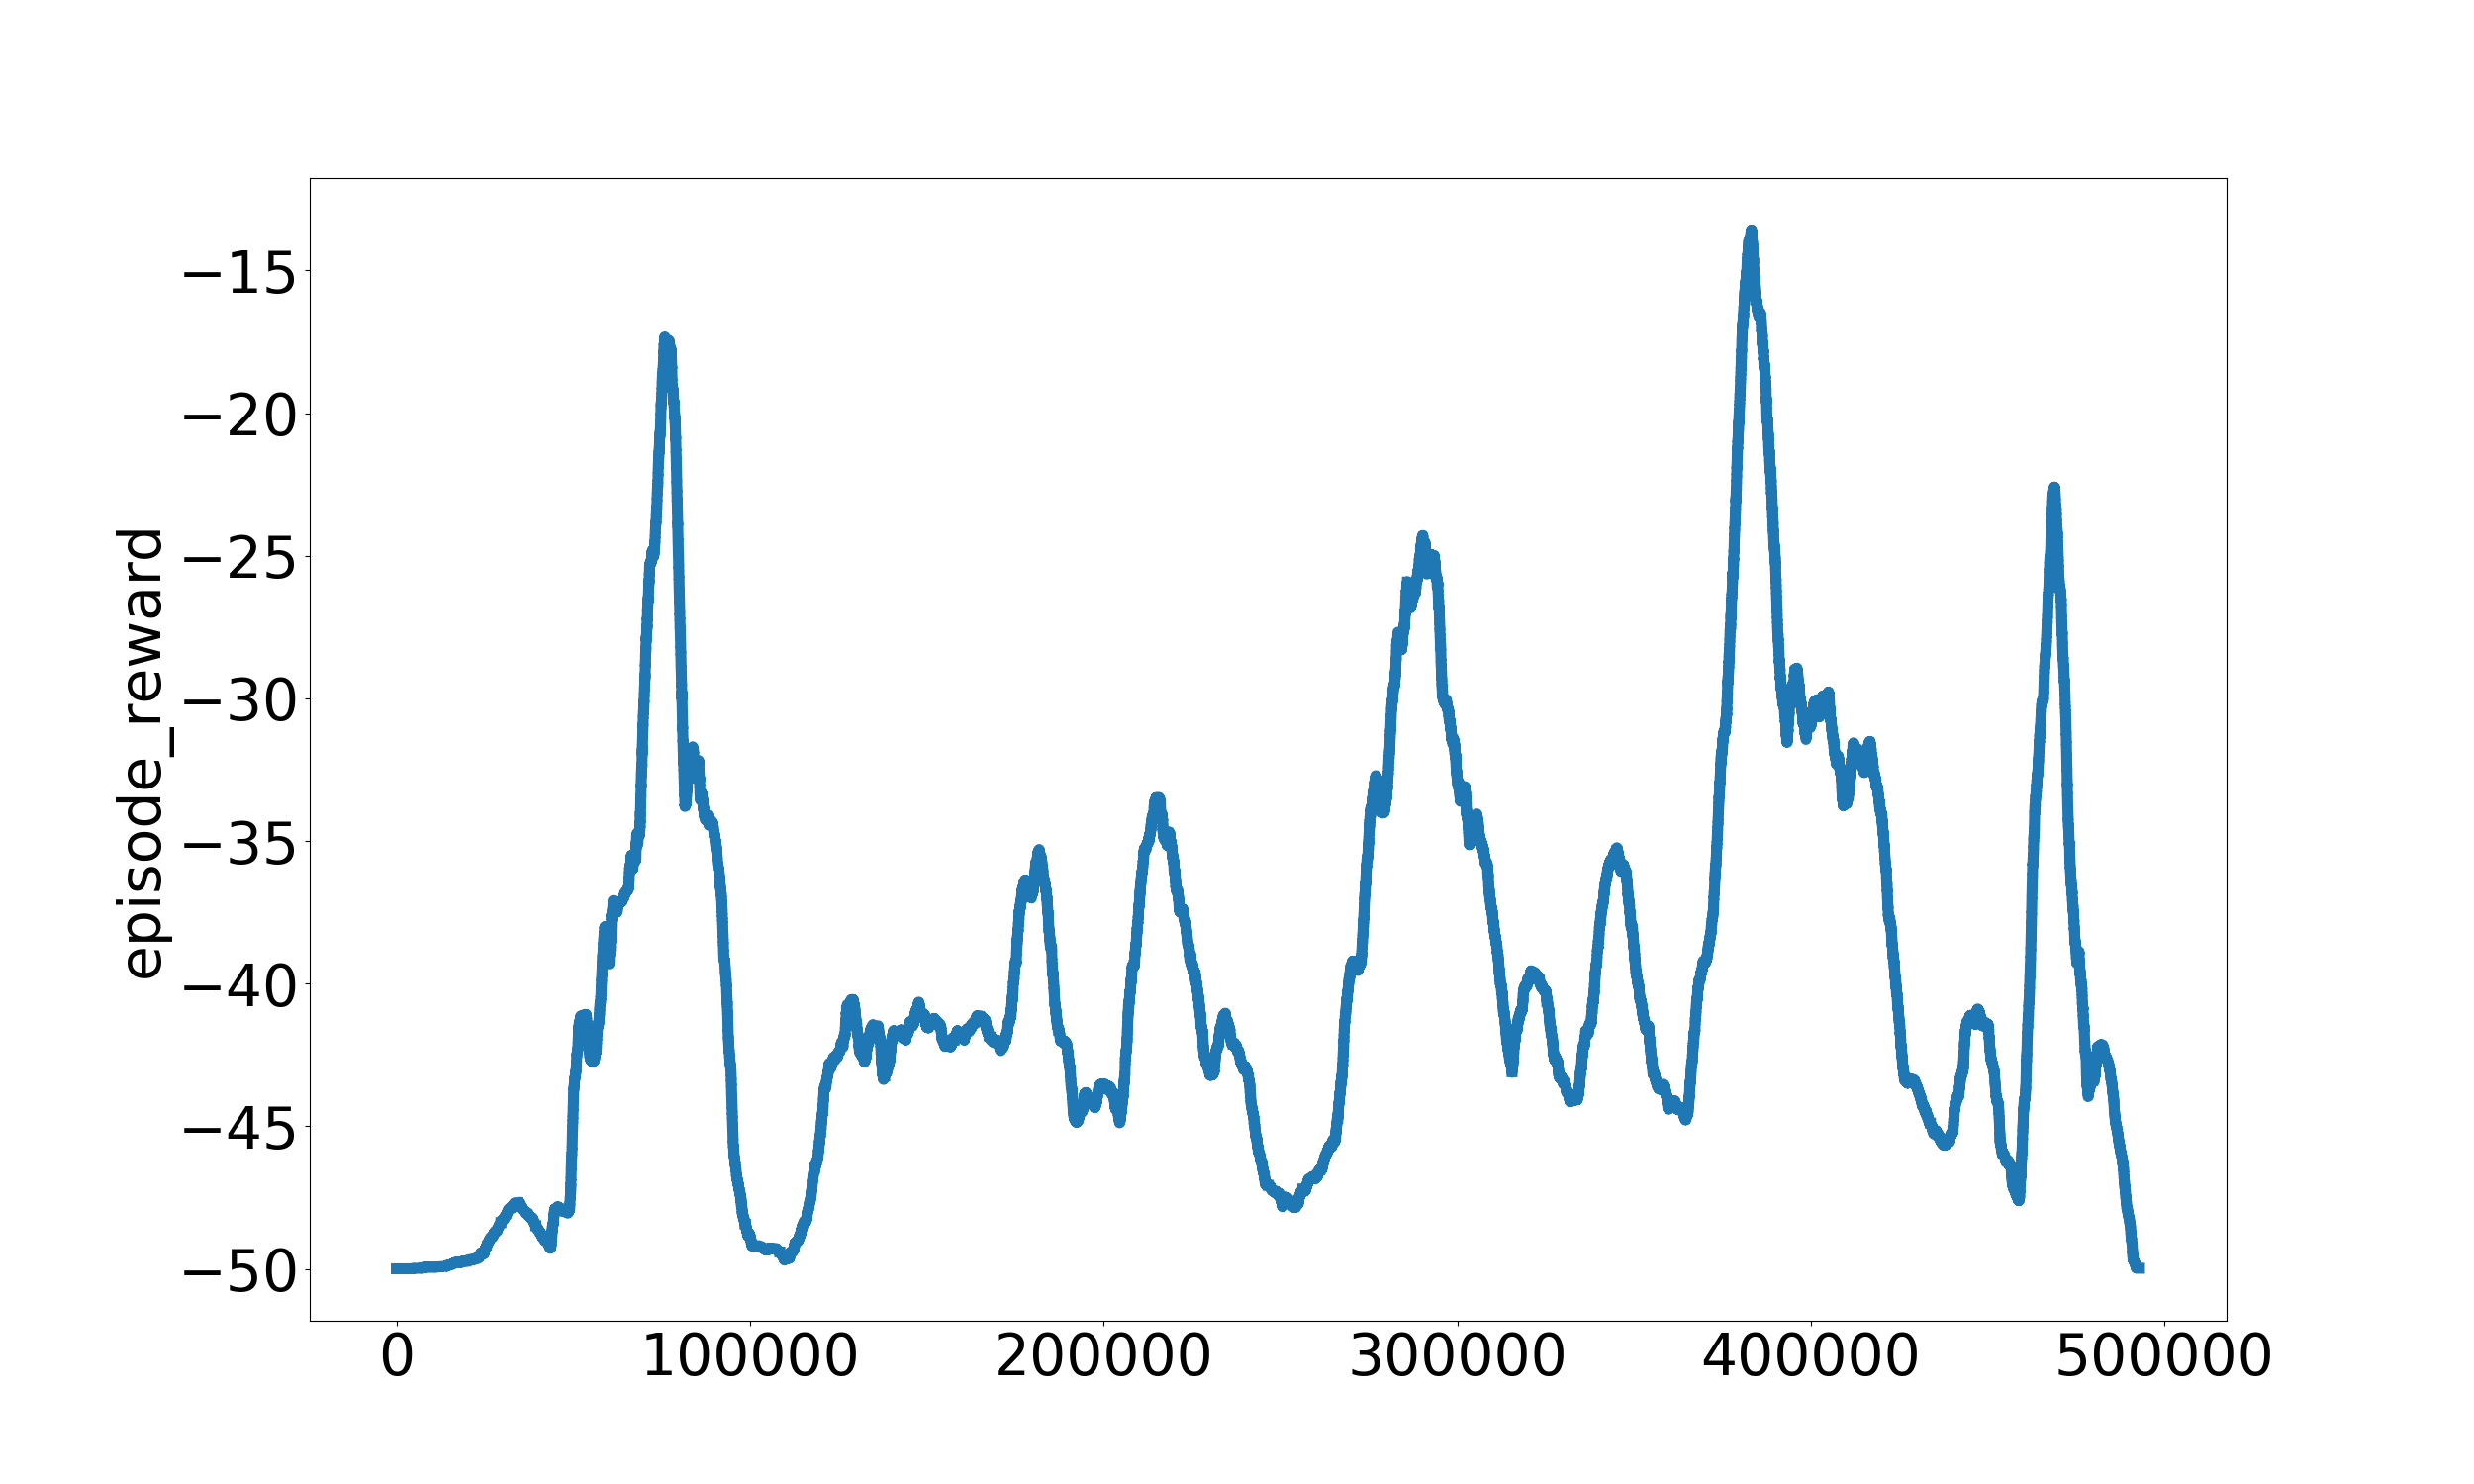
\includegraphics[width=1.1\textwidth]{Pic/baseline/episode_reward.png}  
      \caption{Trung bình tích lũy phần thưởng}
      \label{fig:baseline_avg}
    \end{subfigure}%
    \begin{subfigure}{.5\textwidth}
      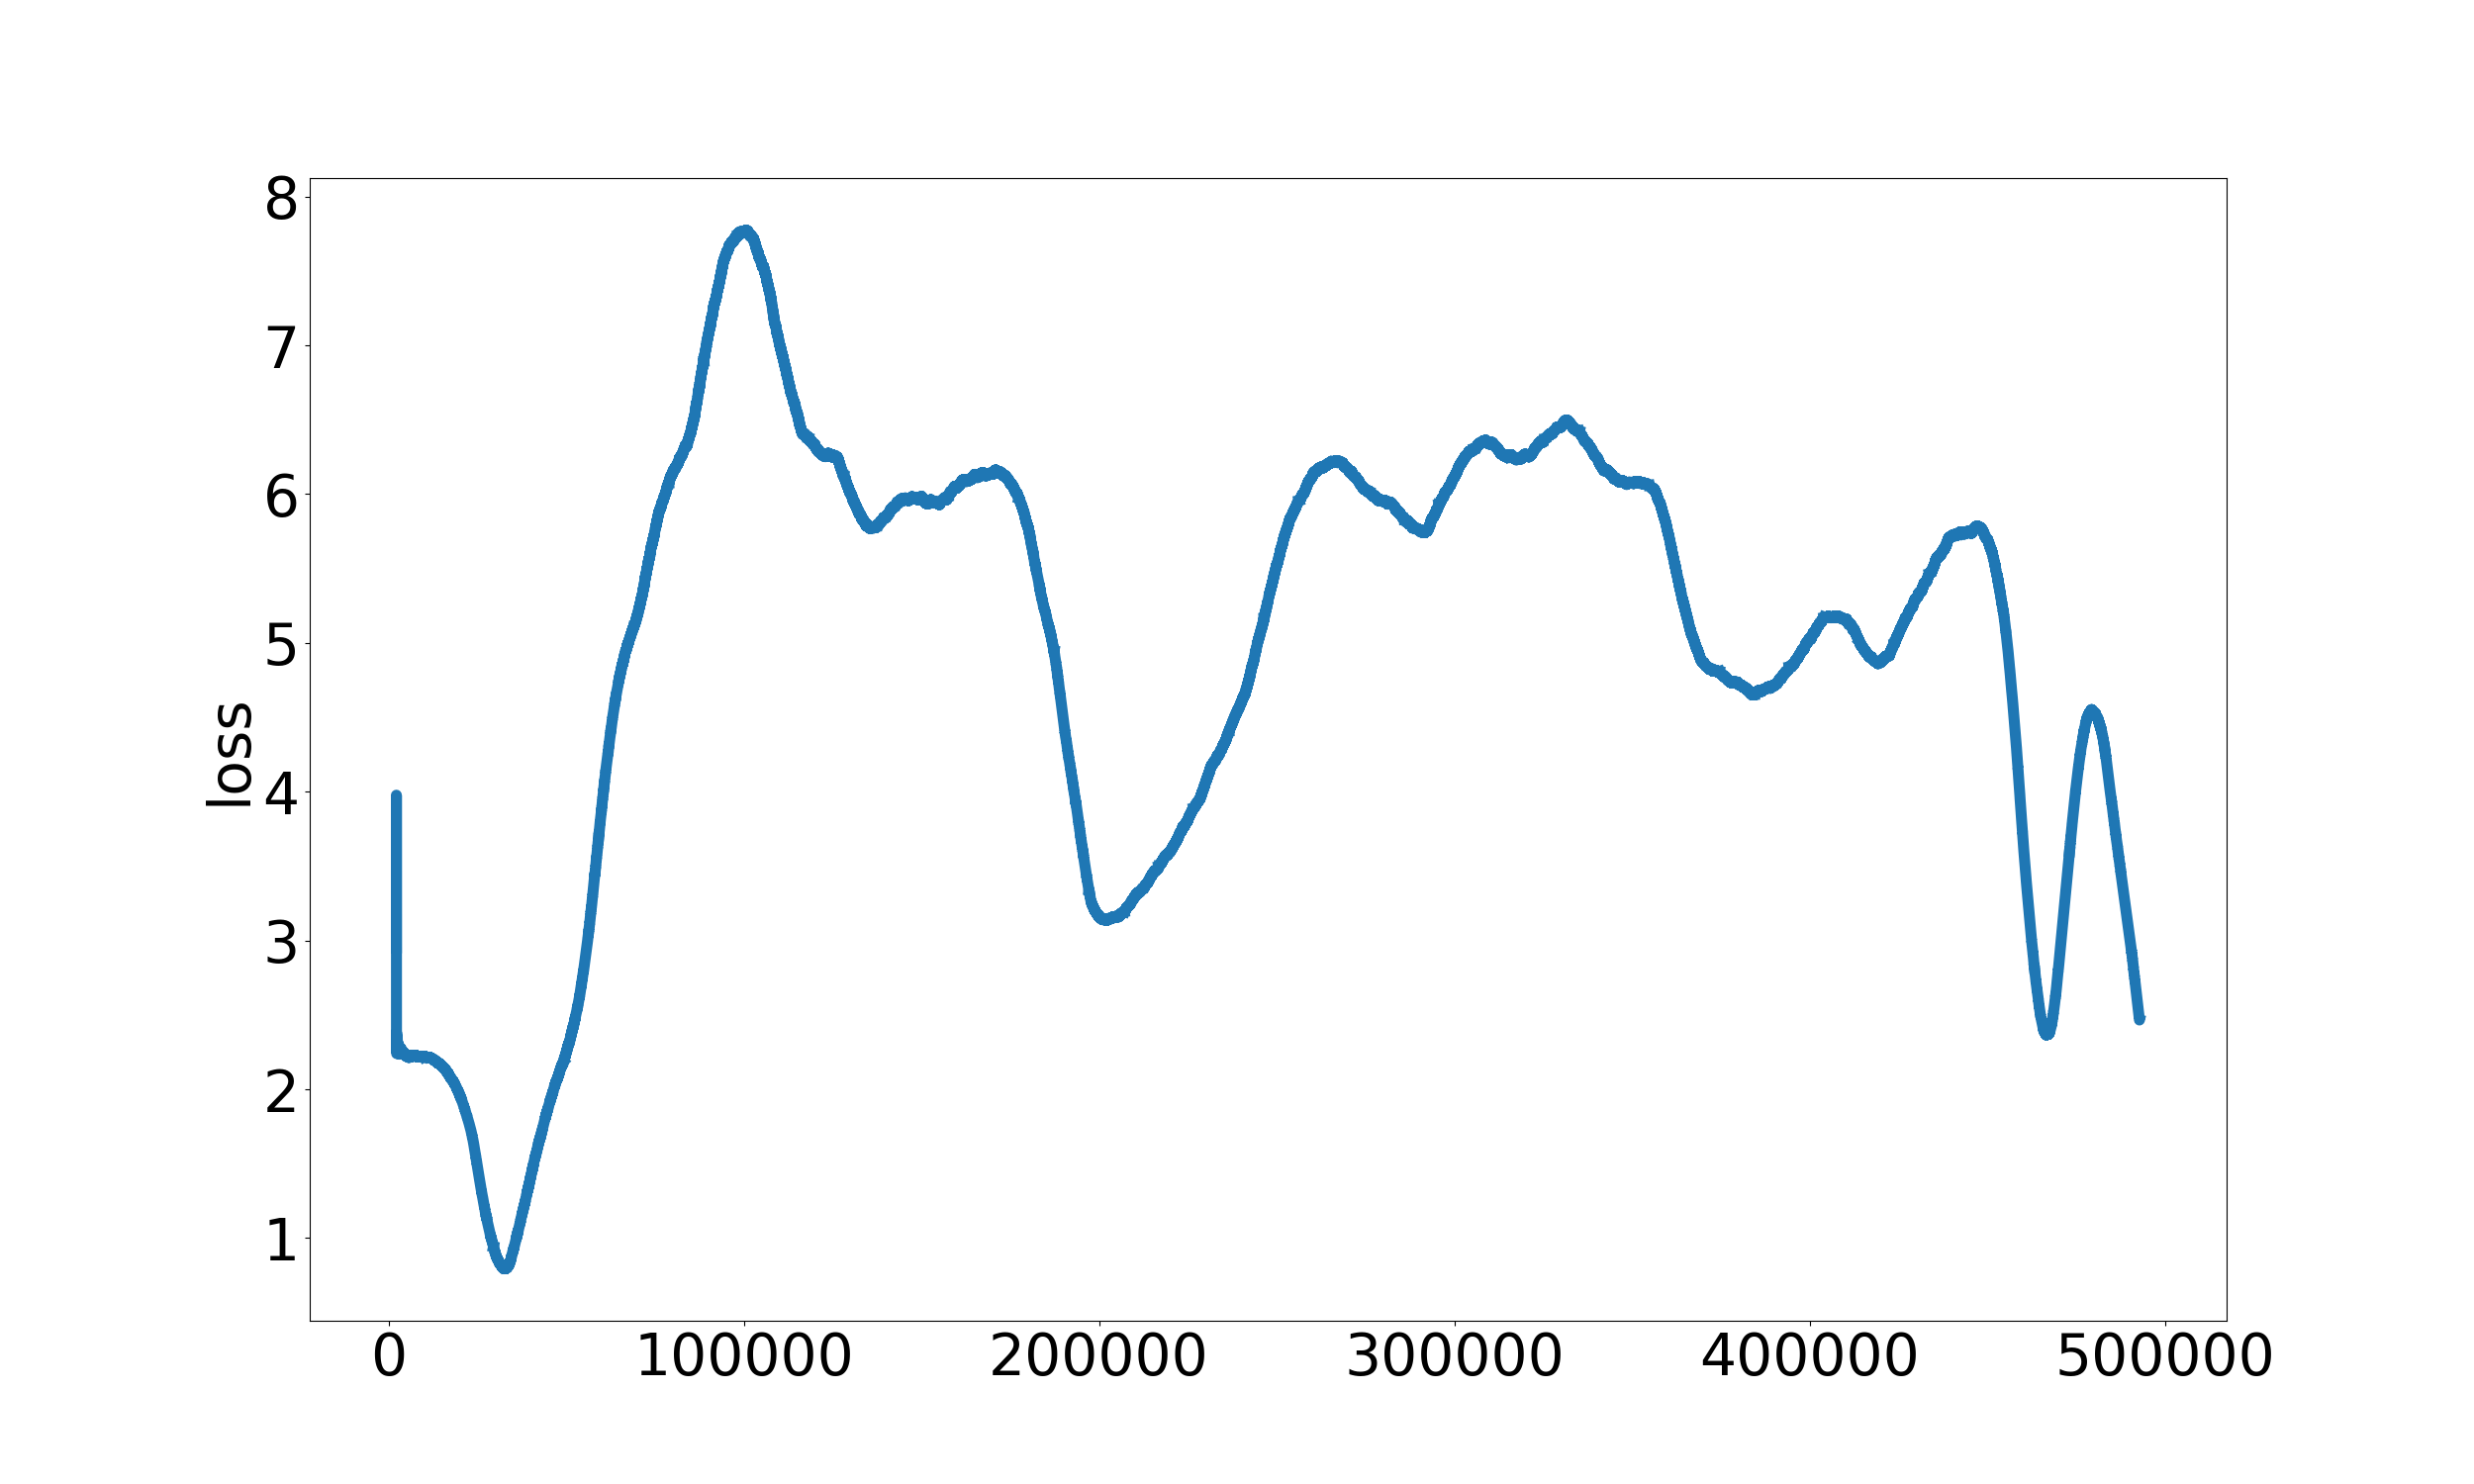
\includegraphics[width=1.1\textwidth]{Pic/baseline/loss.png}  
      \caption{Hàm mất mát}
      \label{fig:baseline_loss}
    \end{subfigure}\\
    \begin{subfigure}{.5\textwidth}
      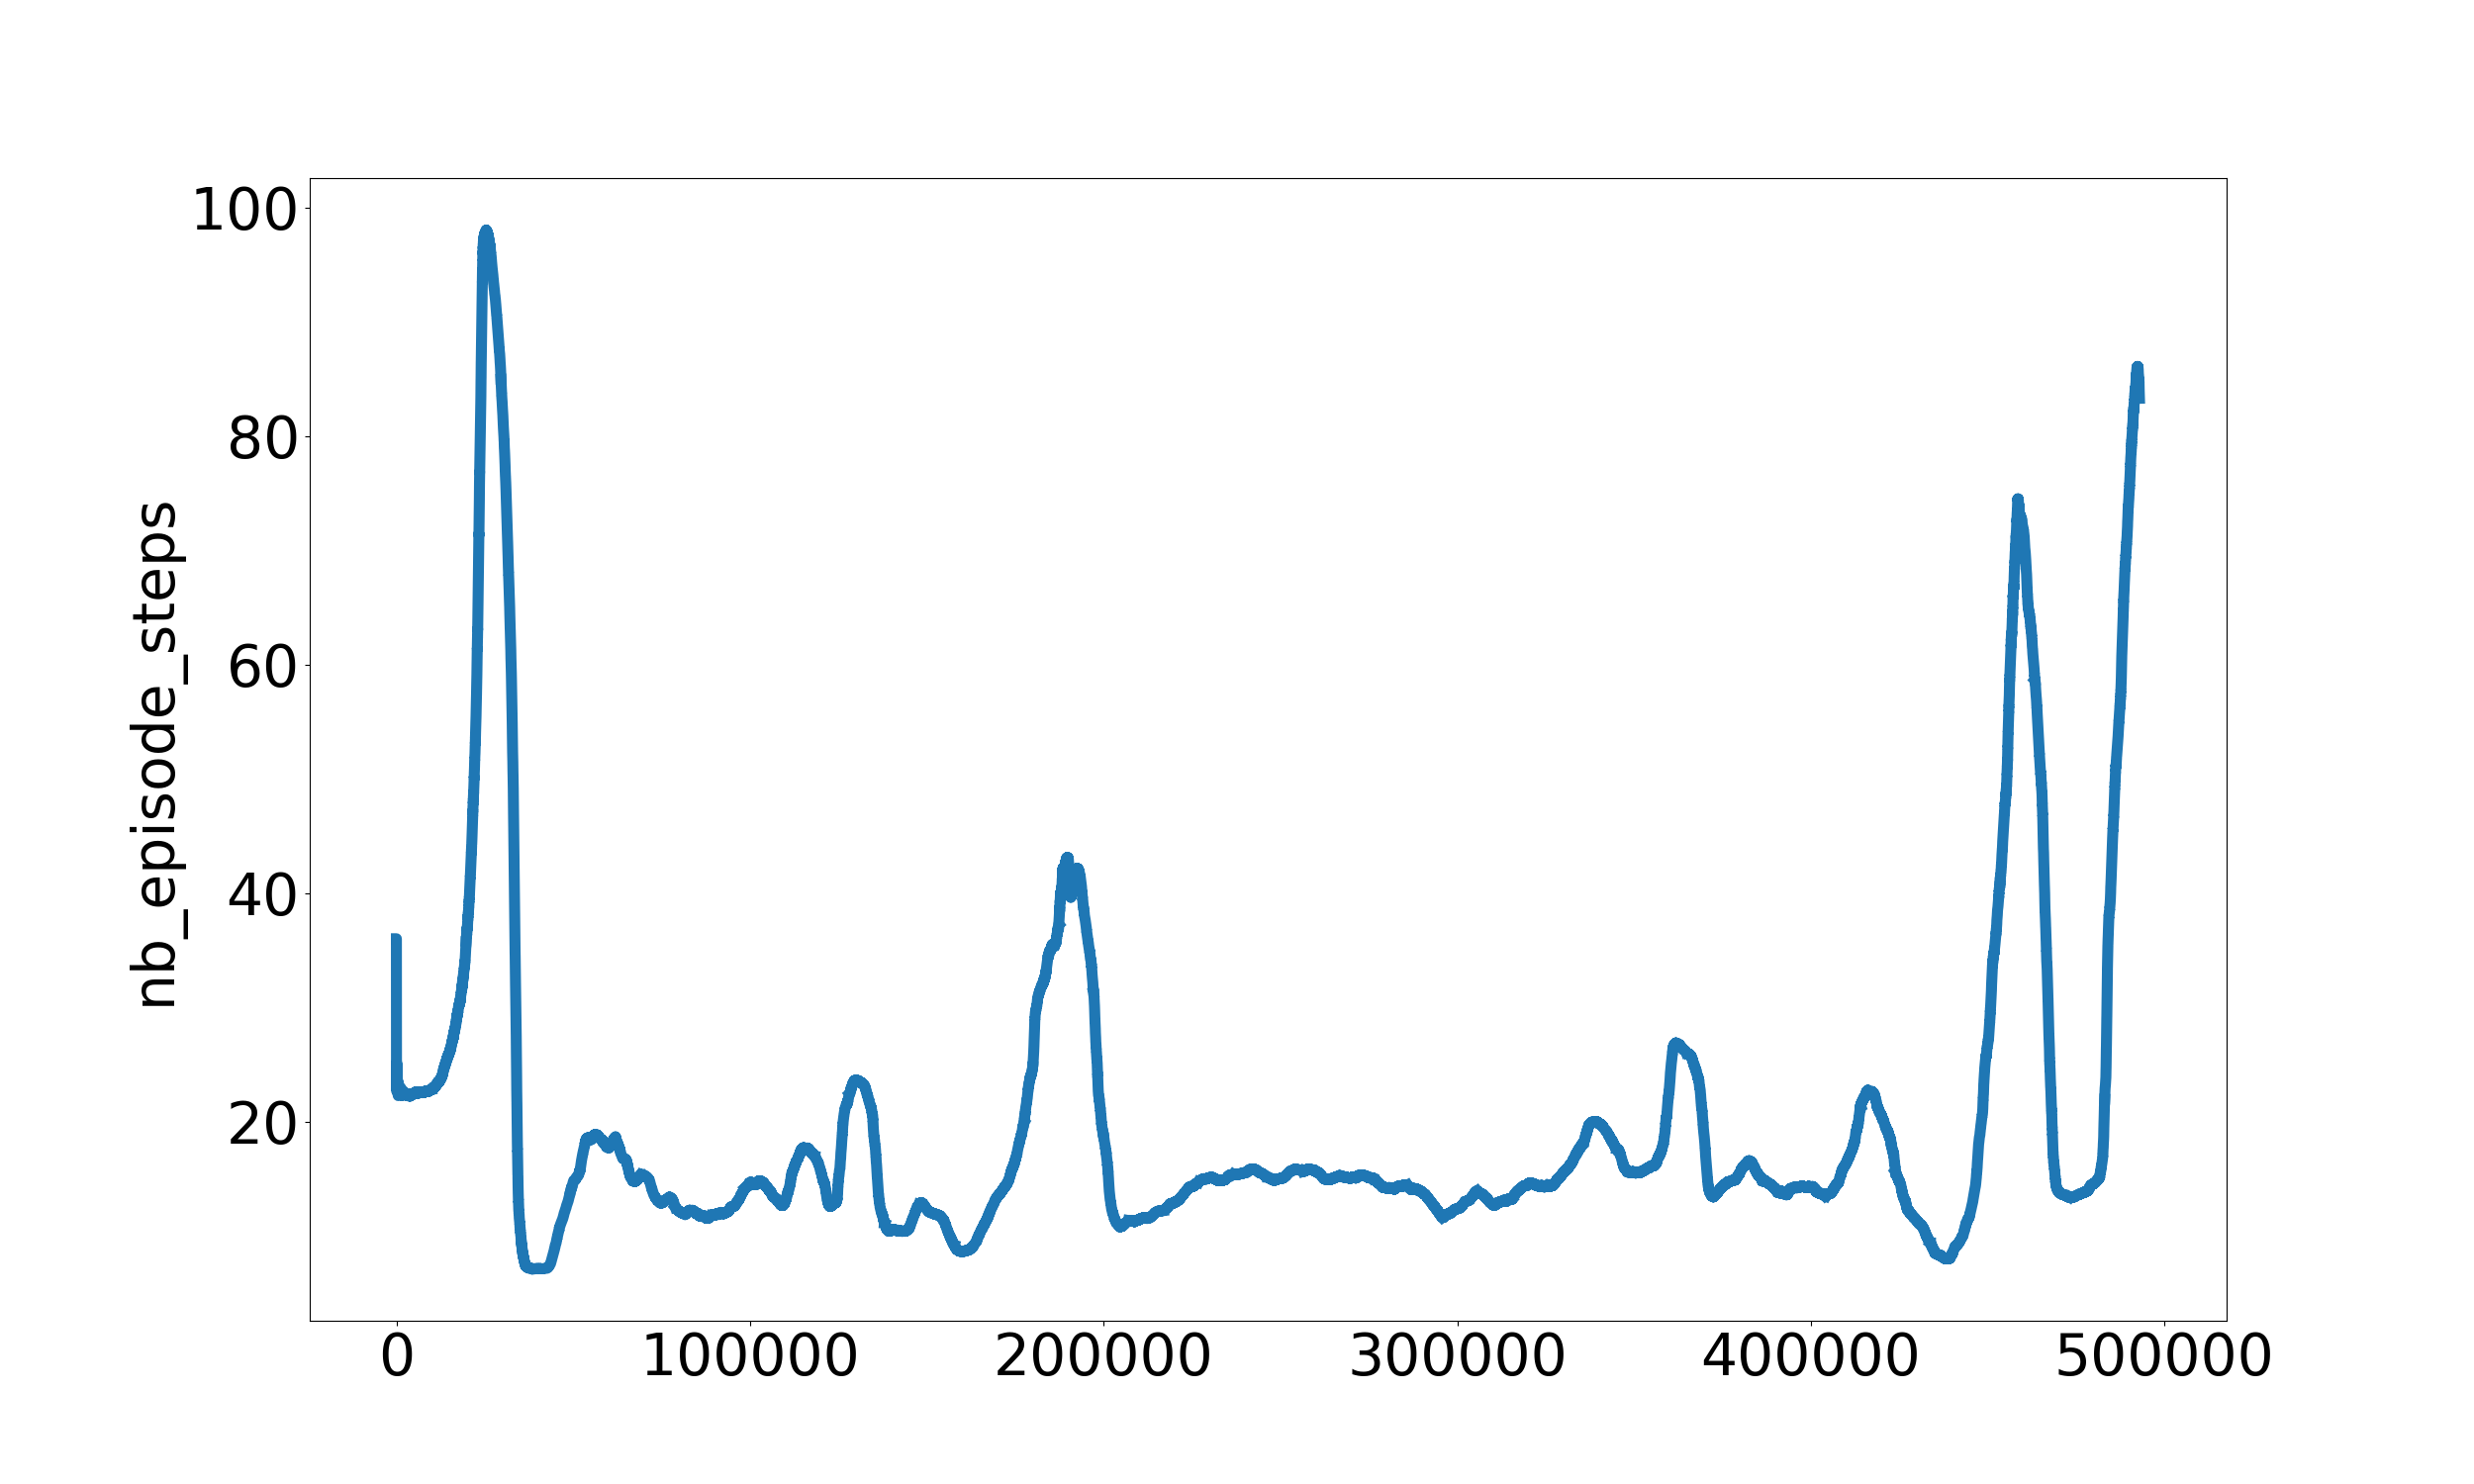
\includegraphics[width=1.1\textwidth]{Pic/baseline/nb_episode_steps.png}
      \caption{Số bước thực hiện}
      \label{fig:baseline_step}
    \end{subfigure}%
    \begin{subfigure}{.5\textwidth}
      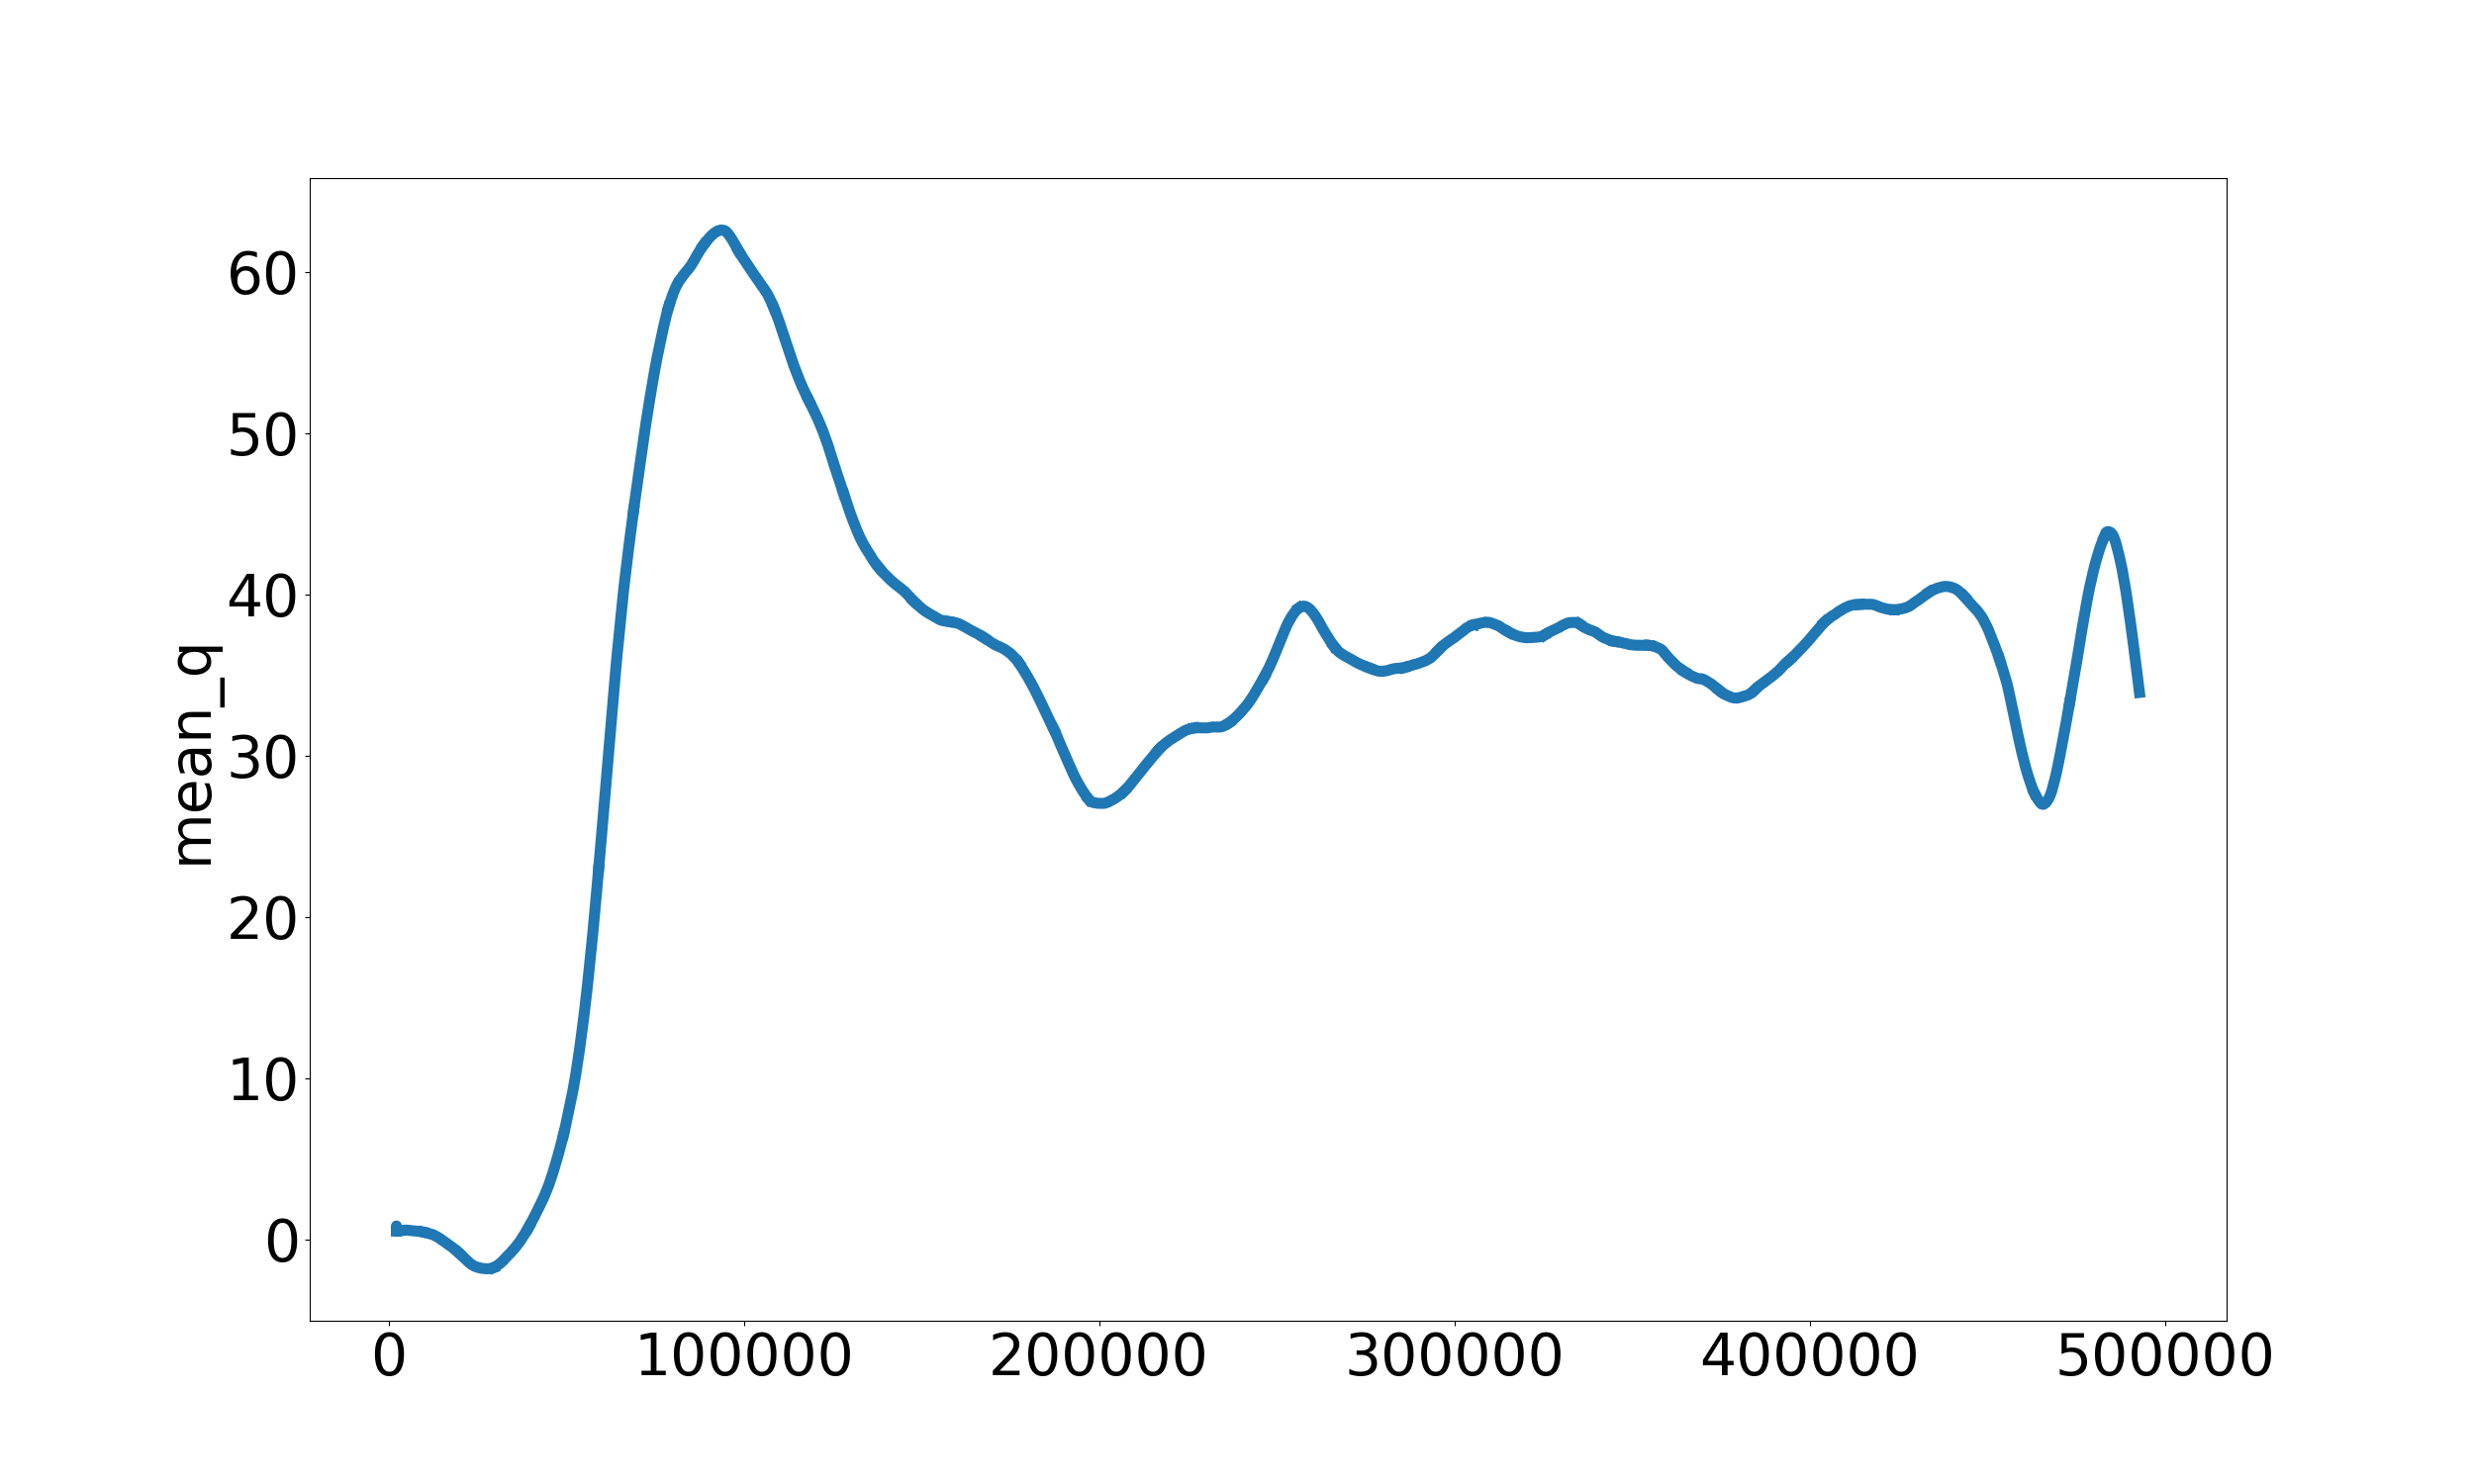
\includegraphics[width=1.1\textwidth]{Pic/baseline/mean_q.png}  
      \caption{Trung bình giá trị Q}
      \label{fig:baseline_mean_q}
    \end{subfigure}
\caption[Kết quả của mô hình cơ sở]{\textit{Kết quả của mô hình cơ sở}, biểu thị quá trình huấn luyện của mô hình. Lưu ý rằng các kết quả được lấy trung bình 10000 tập trước đó để độ thị trông mượt hơn và cảm nhận xu hướng mô hình hoạt động tốt hơn.}
\label{fig:result_baseline}
\end{figure}
\clearpage
\section{Một số thử nghiệm được thực hiện}
\subsection{Mô hình đầu tiên}
\subsubsection{Lần 1}\label{first_model:first_try}
Sau đây là kết quả nhóm thu được khi thực hiện huấn luyện mô hình \ref{first_model} trong 14M bước được thực thi. Hàm phần thưởng được sử dụng cho lần thực nghiệm là:
    \begin{subnumcases}{r(s_t,a_t,s_{t+1})=}
        +10 & $s_{t+1}=\text{đích}$ \\
        -10 & $s_{t+1}=\text{chết}$\\
        -\frac{15-\text{vị trí robot}}{15- 4} & \text{còn lại}\label{first_subtract_10}
    \end{subnumcases}
Có thể thấy các thay đổi mô hình đã có tín hiệu tích cực khi hình \ref{fig:result_first_model:try_1} cho thấy mô hình đã đáp ứng hết các kỳ vọng được đưa ra. Phần thưởng trung bình tích lũy của 10000 trong tập hình  \ref{fig:first_model:try_1:avg} đã tăng tuyến tính, mặc dù các giá trị phần lớn bé hơn 0 nhưng có thể giải thích rằng phần thưởng khi chạm đích của robot là nhỏ so với tổng của của lượng âm khi robot thực hiện các bước. Tuy nhiên đồ thị cho thấy phần thưởng tích lũy không vượt lên được nữa khi trong suốt thời gian huấn luyện các giá trị giao động trong khoảng -7, vì hình phạt mỗi lần robot thực hiện bước đi lớn nhất là bé hơn một nên kết quả này có thể là tín hiệu đáng mừng. Để kiểm tra kết quả đạt được, tỷ lệ thắng đạt \textbf{50.6\%} trường hợp robot thắng. Giả thiết rằng có rất nhiều trường hợp robot chưa gặp phải hoặc có rất nhiều trạng thái chưa được cập nhật đủ.\\
\\
Dựa trên hình \ref{fig:first_model:try_1:loss}, các giá trị chỉ dao động quanh giá trị 4 trong phần lớn thời gian huấn luyện, có thể mô hình không thể tìm được chính sách khác có thể để thỏa mãn hết mọi trạng thái của môi trường. Giả thiết rằng khi thực hiện ngẫu nhiên vị trí của robot sẽ khiến mỗi lần cập nhật xác suất cao có cả cập nhật trường hợp thắng nhiều, điều này có thể là cản trở cho việc thử các chính sách khác của mô hình.\\
Kết quả so sánh giữa đồ thị \ref{fig:baseline_step} và đồ thị \ref{fig:first_mode:try_1:step} cho thấy rằng việc thay đổi hàm phần thưởng âm giúp cho robot không muốn ở lại lâu trên môi trường khi từ khoảng $(0-3000)$, các bước cần thực hiện trong mỗi tập giảm còn trong khoảng $(0-300)$.
\clearpage
\begin{figure}[hb]
    \centering
    \begin{subfigure}{.5\textwidth}
      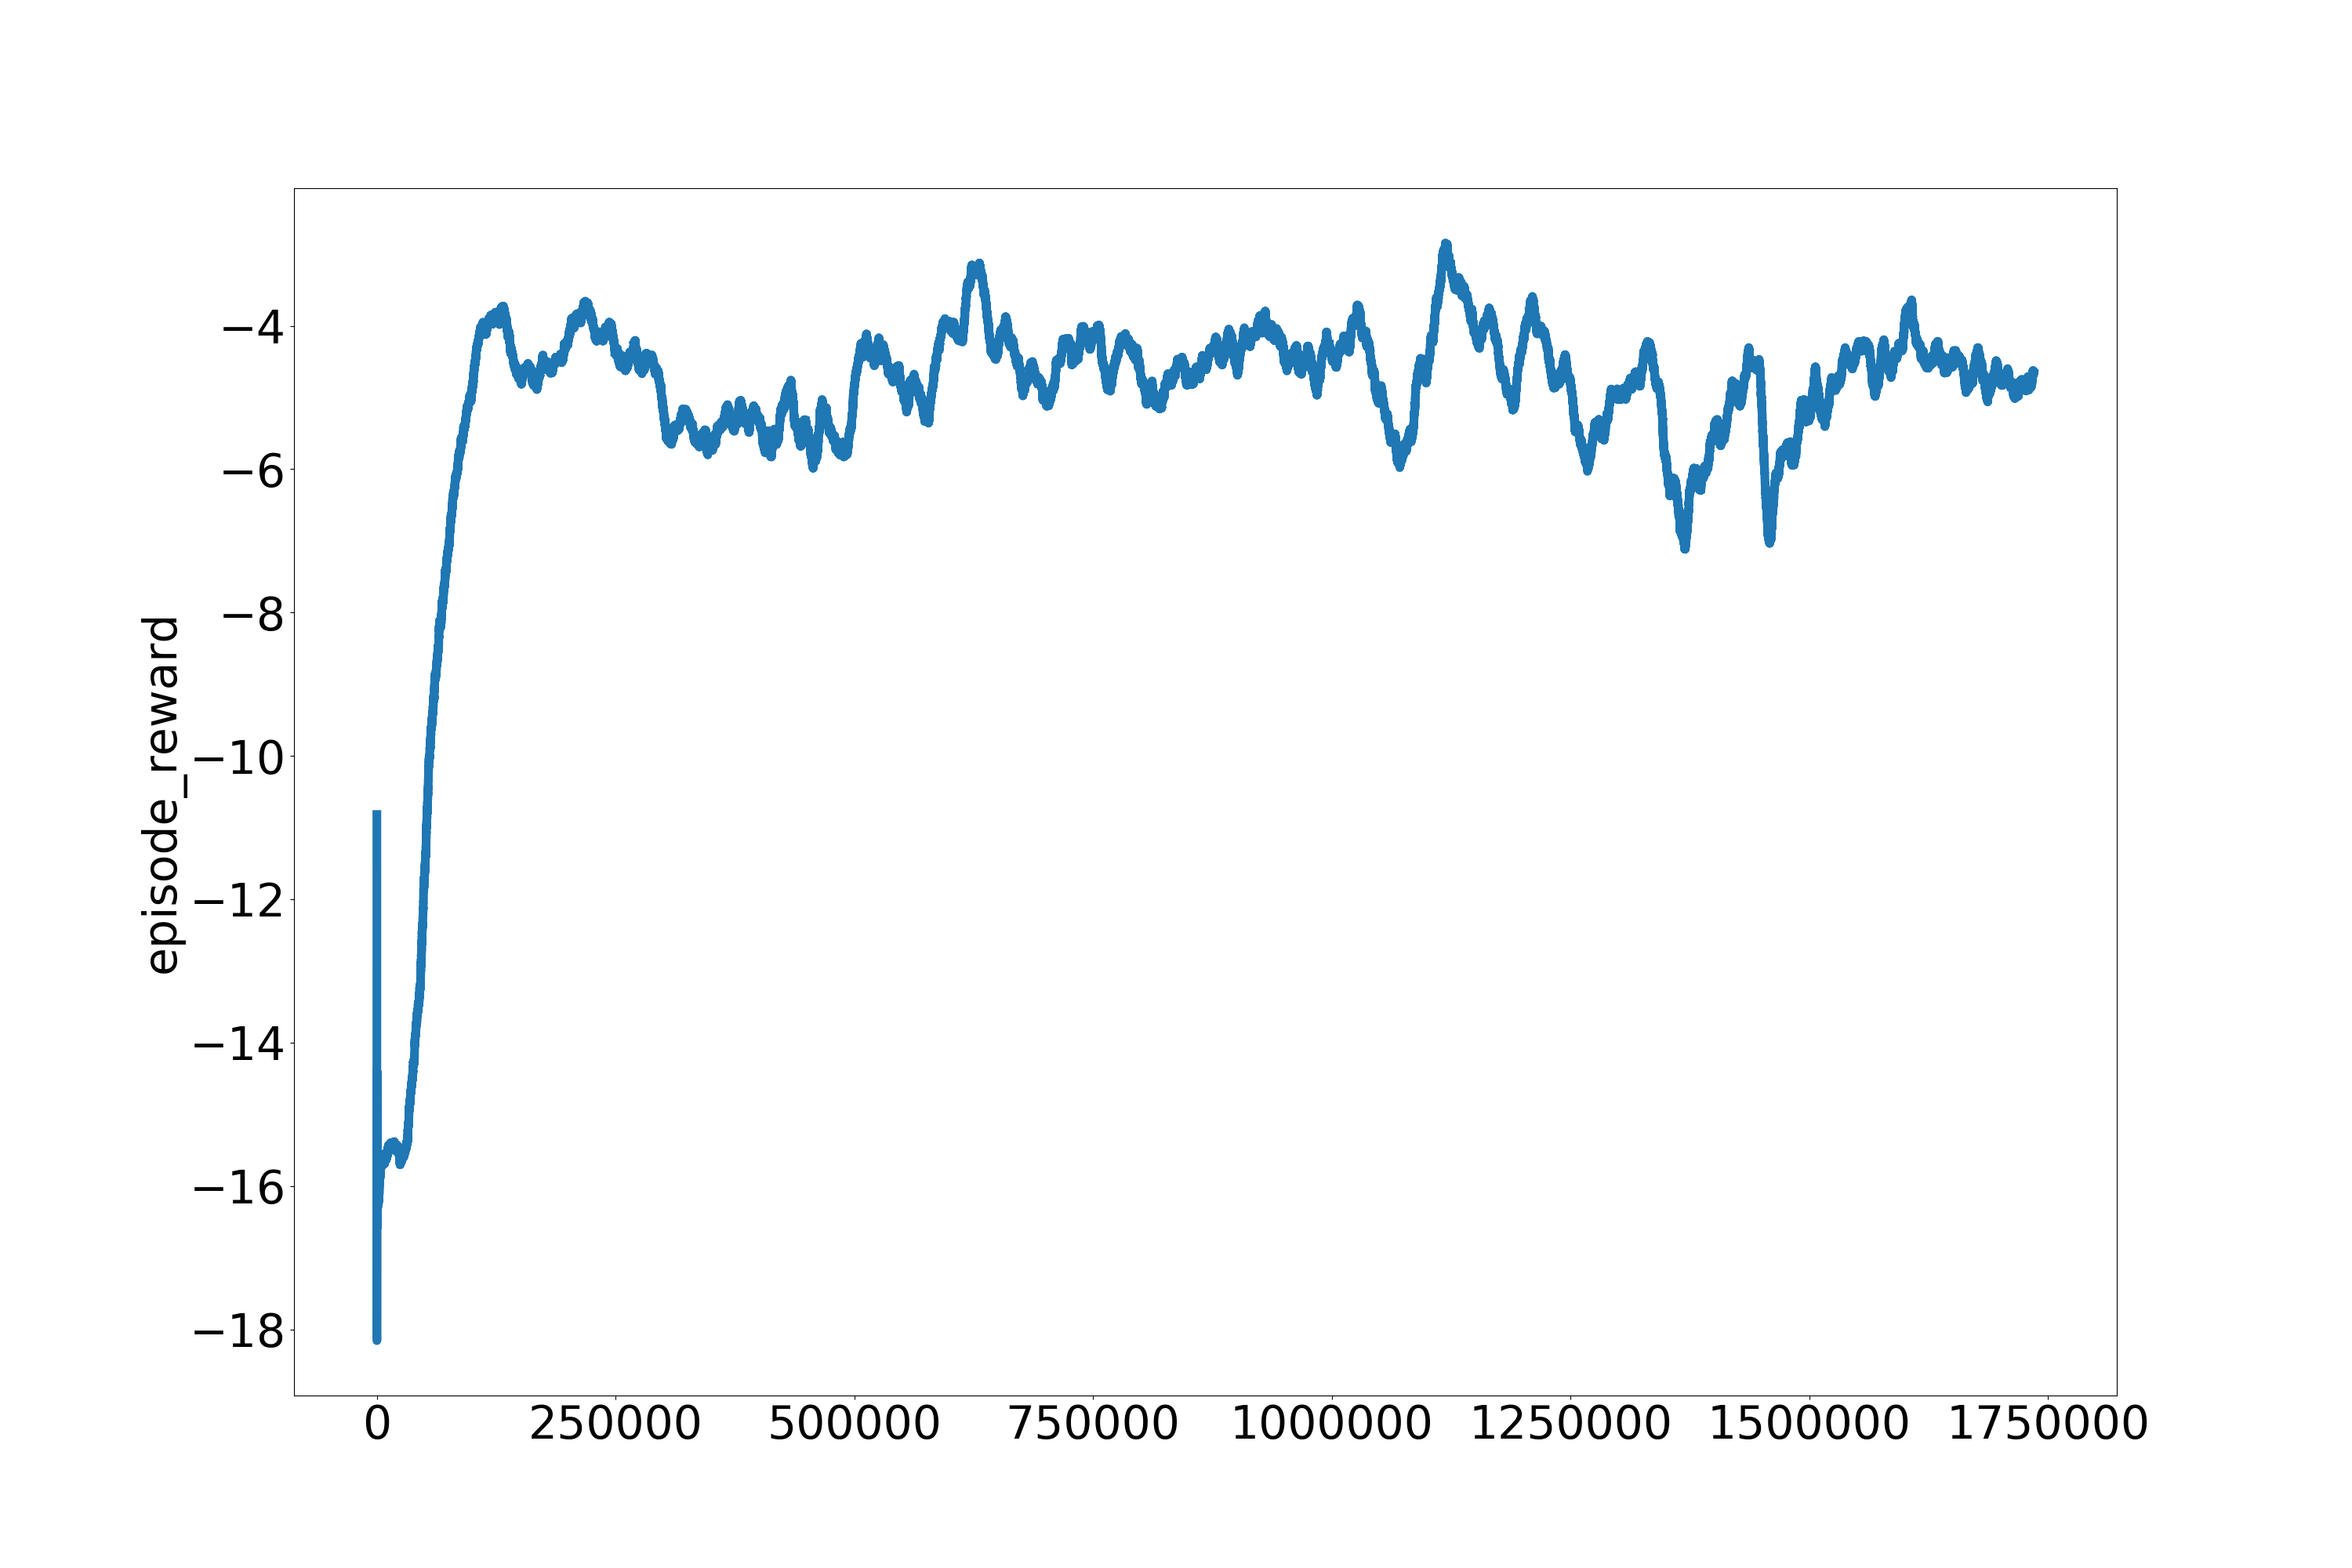
\includegraphics[width=1.1\textwidth]{Pic/First_model/episode_reward.png}
      \caption{Trung bình tích lũy phần thưởng}
      \label{fig:first_model:try_1:avg}
    \end{subfigure}%
    \begin{subfigure}{.5\textwidth}
      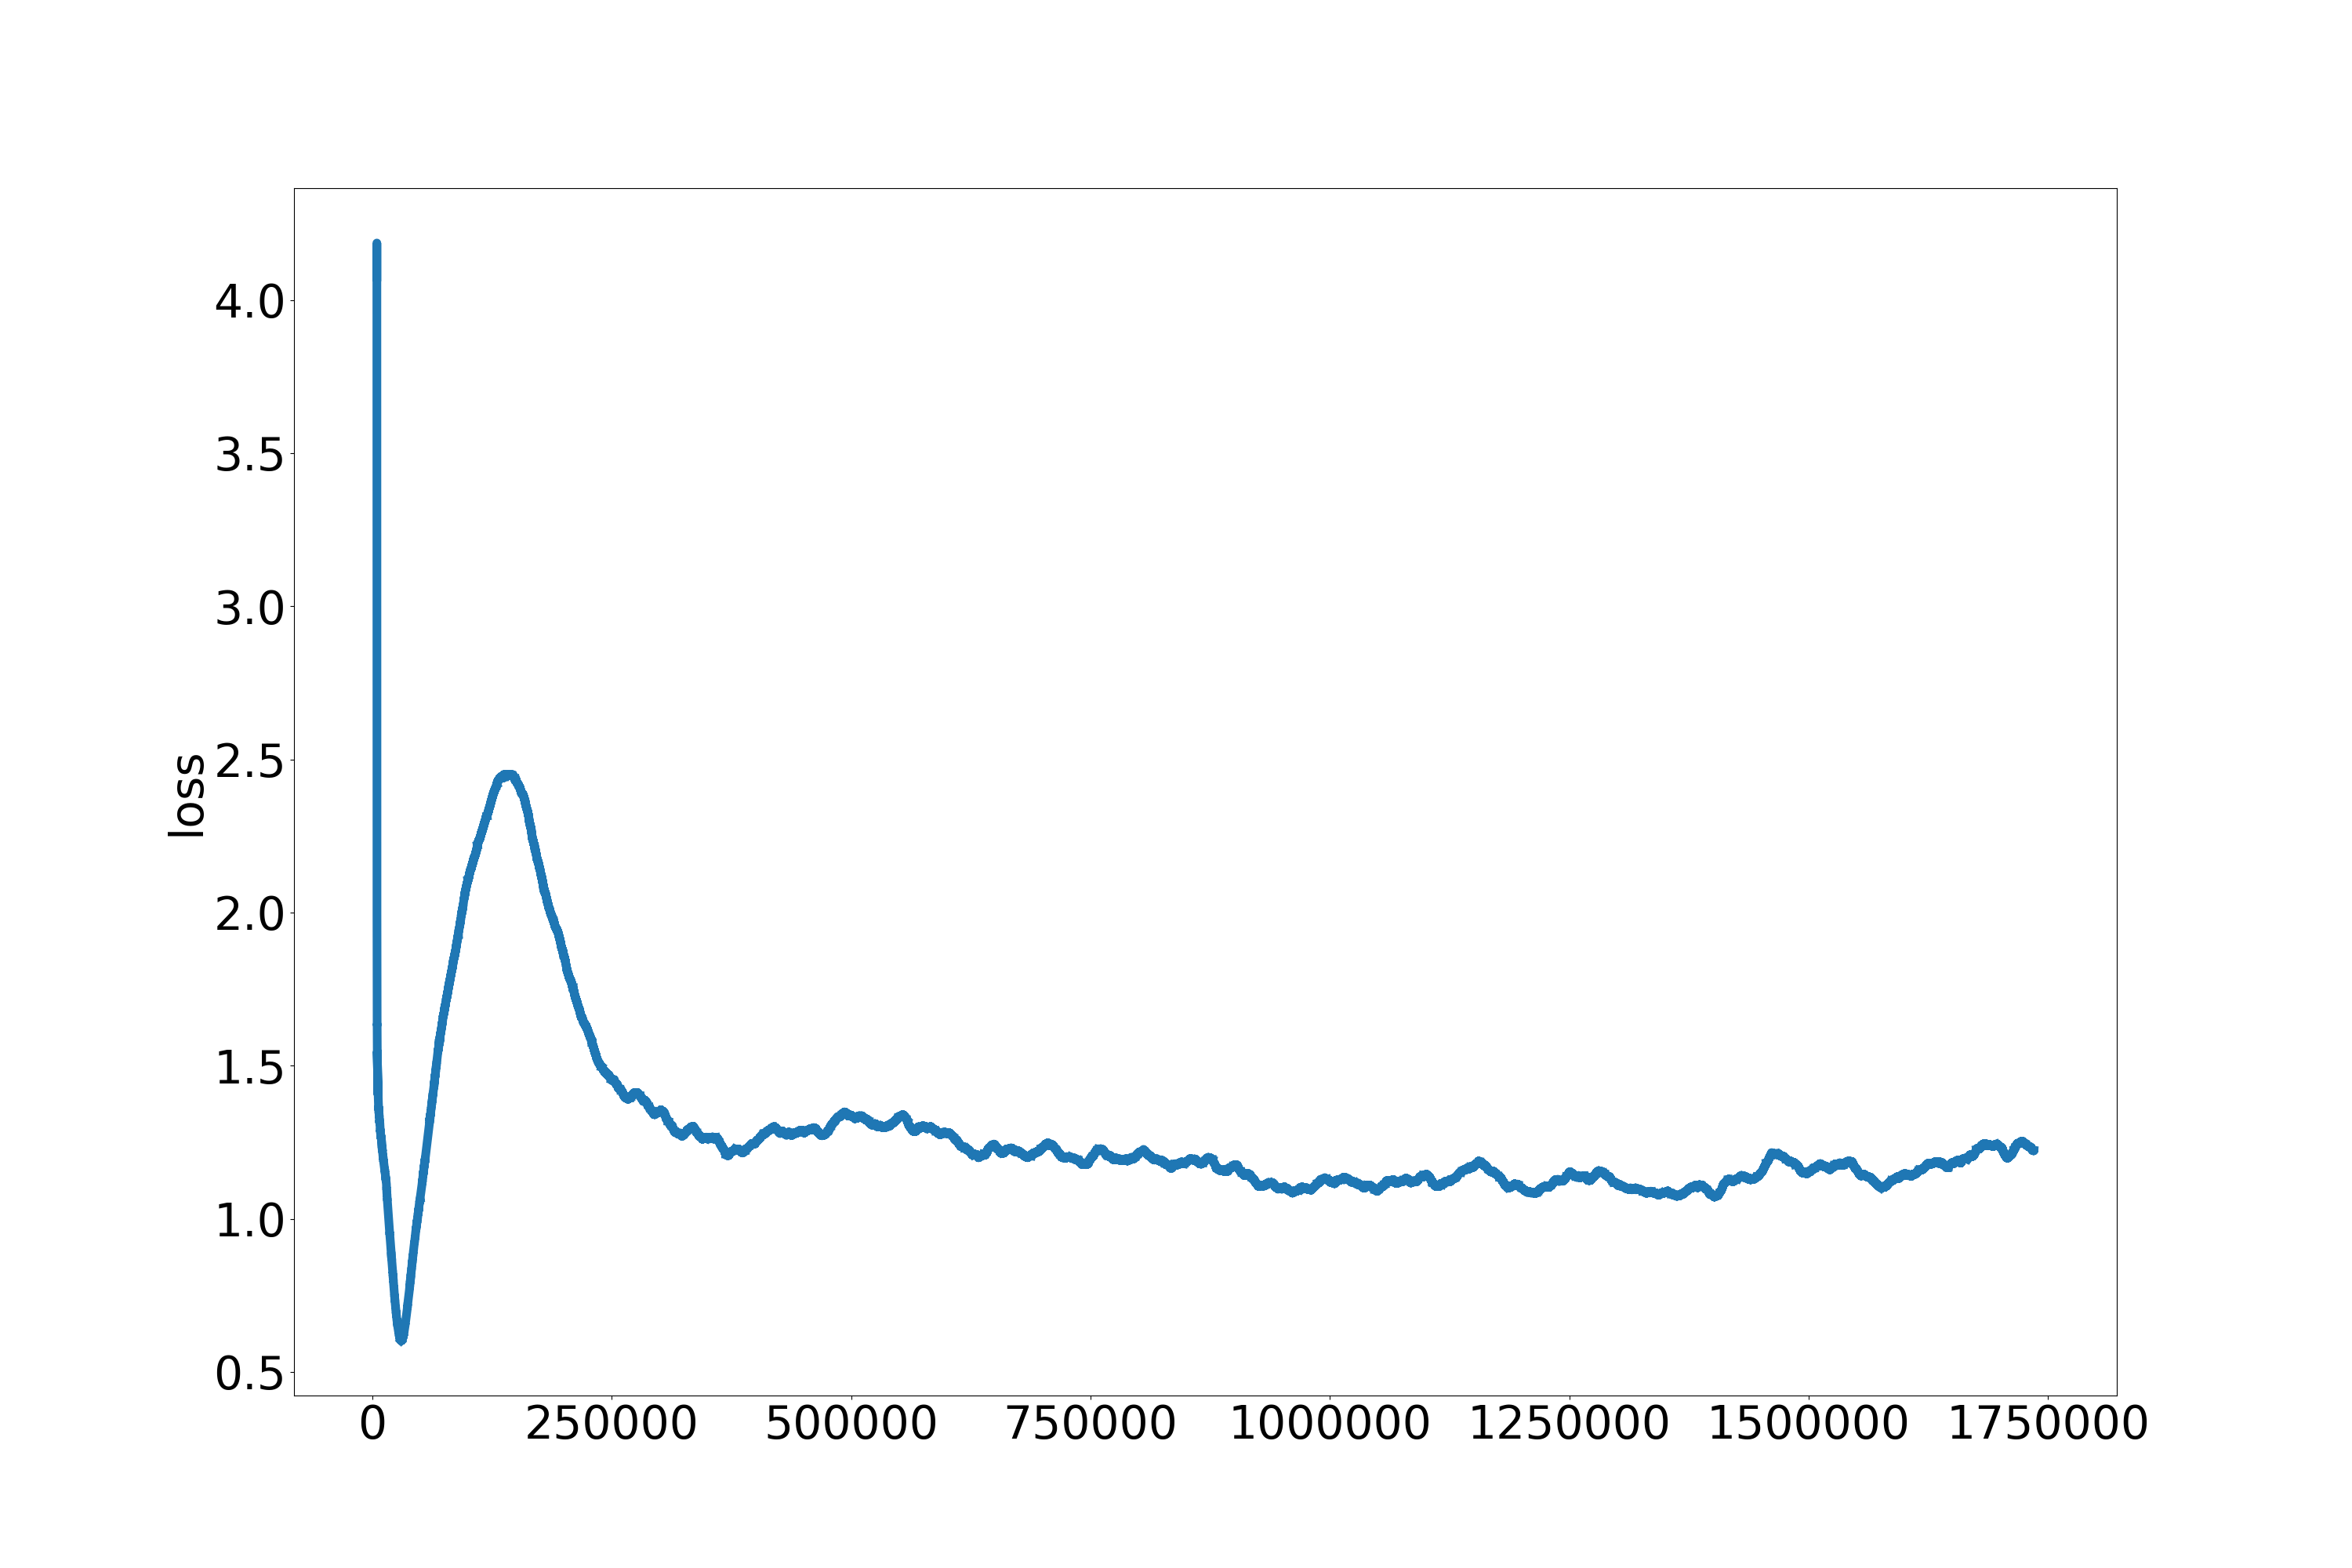
\includegraphics[width=1.1\textwidth]{Pic/First_model/loss.png}
      \caption{Hàm mất mát}
      \label{fig:first_model:try_1:loss}
    \end{subfigure}
    \begin{subfigure}{.5\textwidth}
      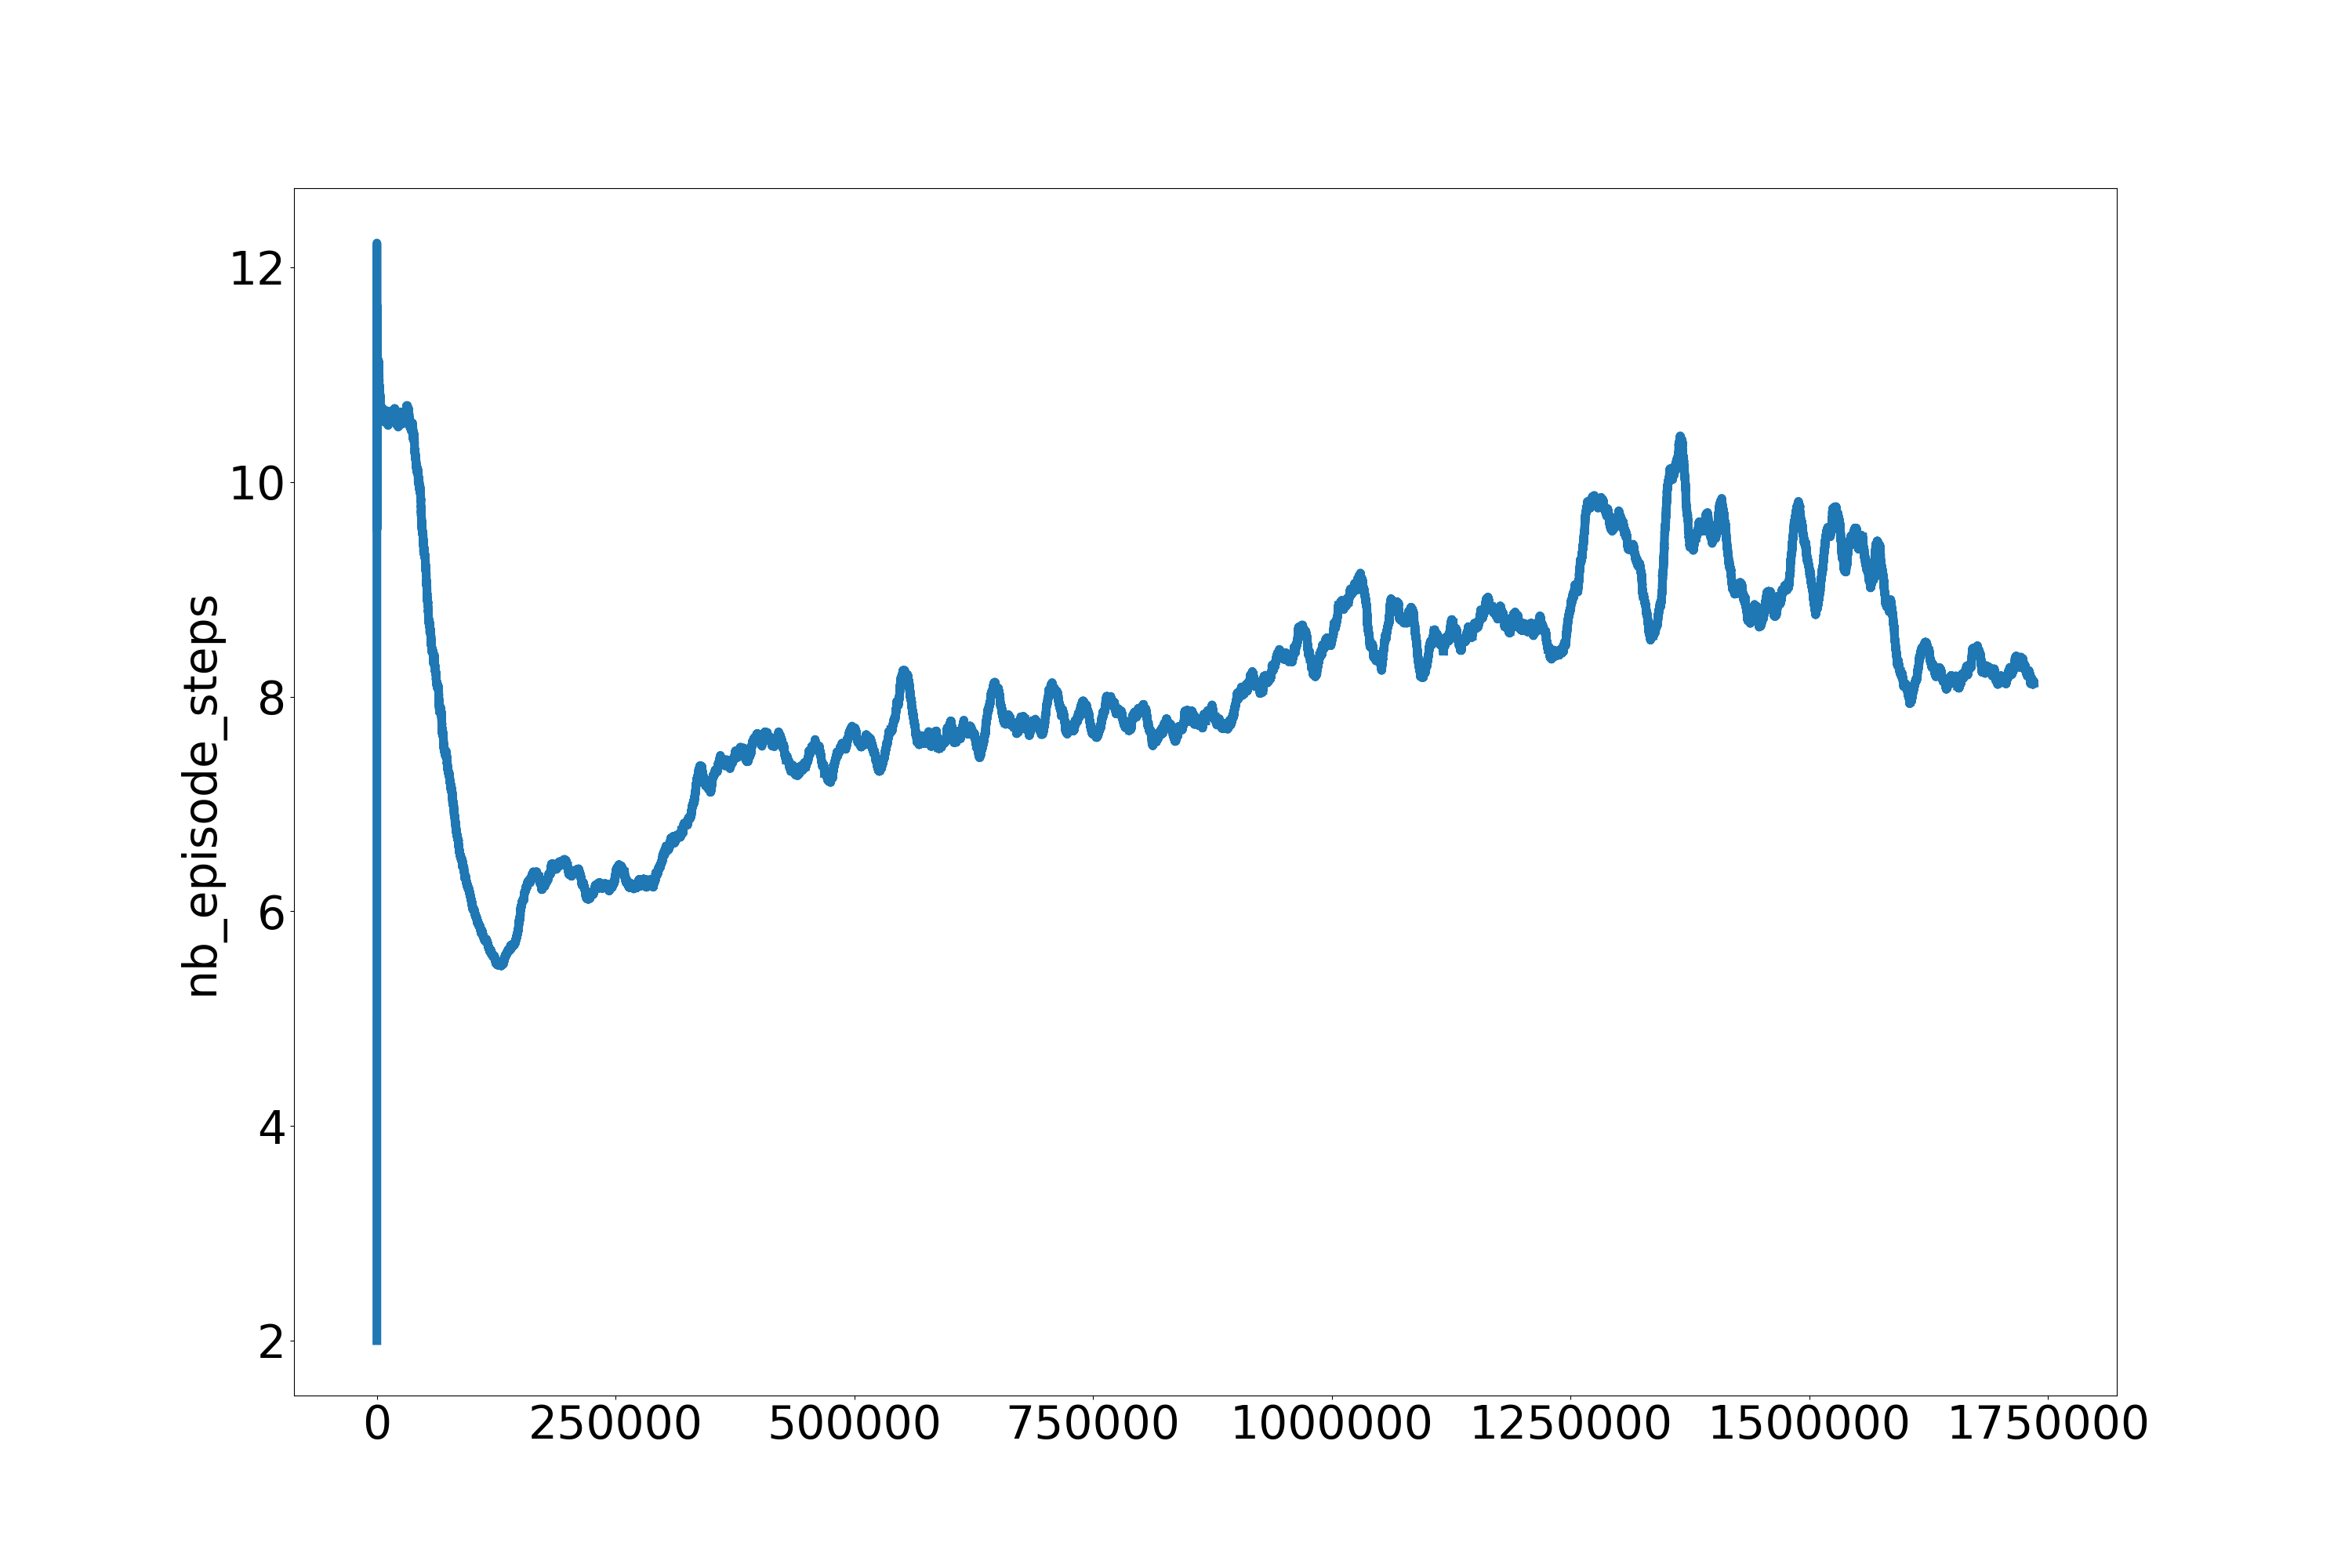
\includegraphics[width=1.1\textwidth]{Pic/First_model/nb_episode_steps.png}
      \caption{Số bước thực hiện}
      \label{fig:first_mode:try_1:step}
    \end{subfigure}%
    \begin{subfigure}{.5\textwidth}
      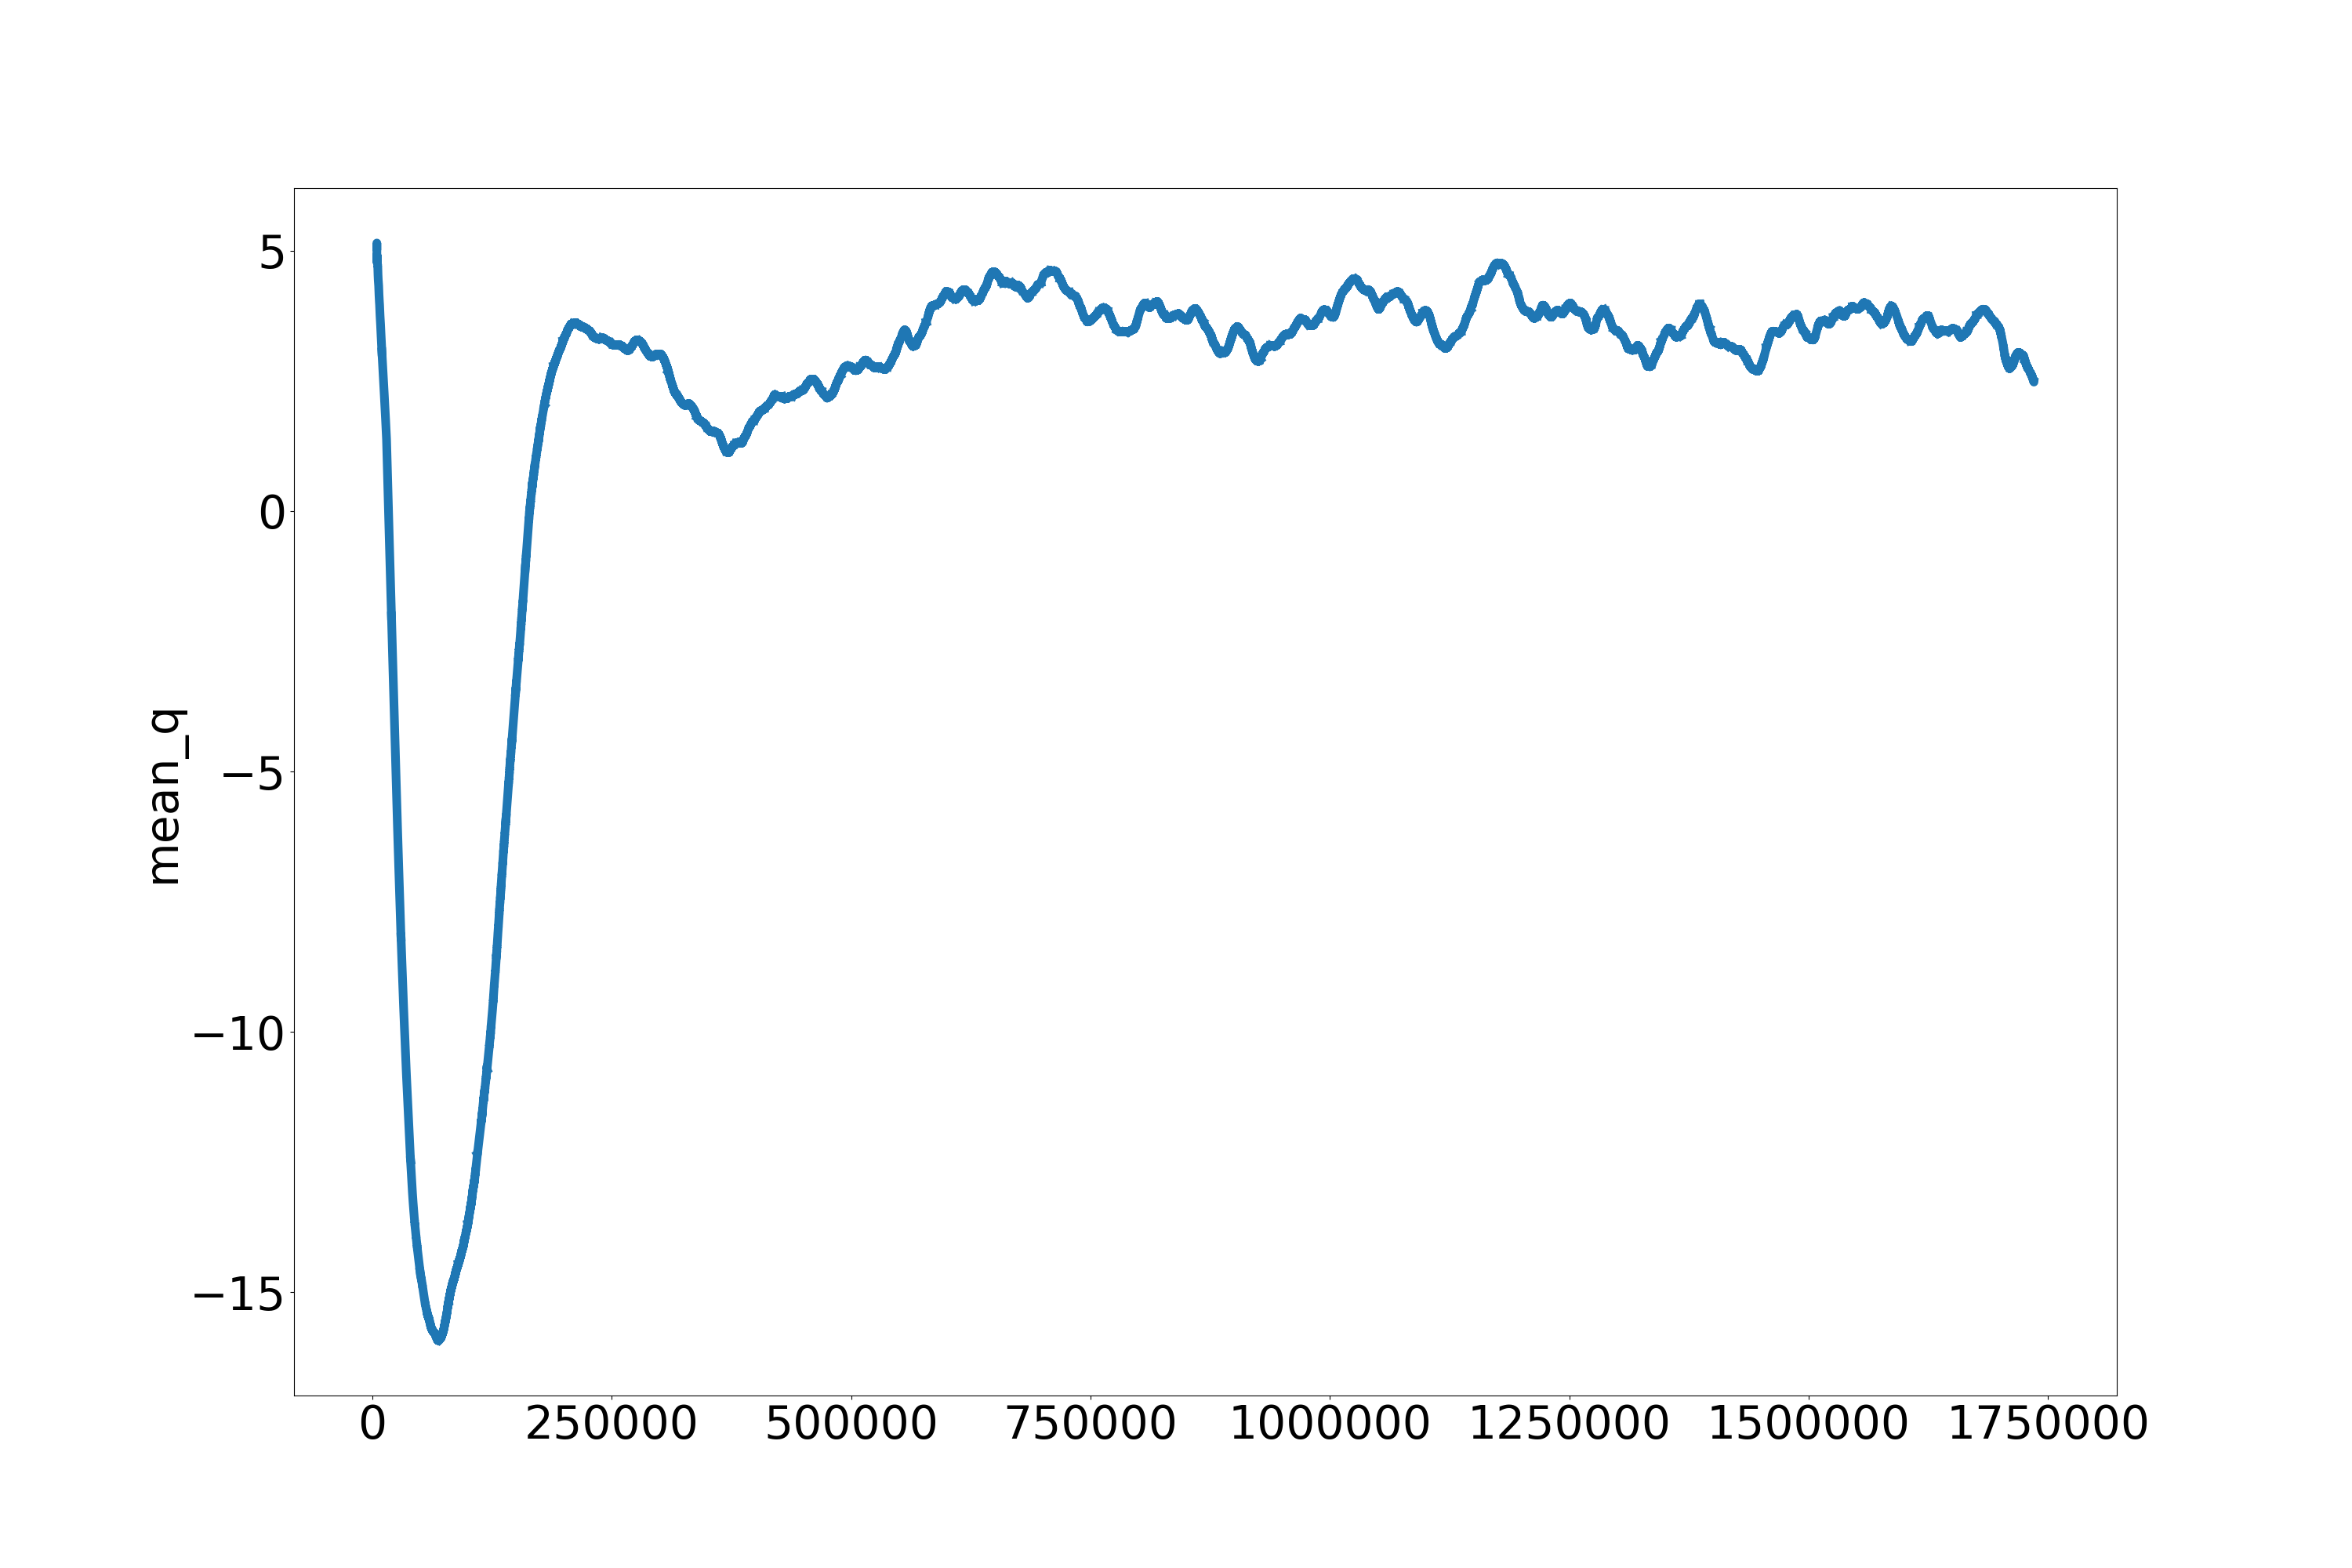
\includegraphics[width=1.1\textwidth]{Pic/First_model/mean_q.png}
      \caption{Trung bình giá trị Q}
      \label{fig:first_model:try1:mean_q}
    \end{subfigure}
\caption[Kết quả của mô hình thứ nhất lần nhất]{\textit{Kết quả của mô hình thứ nhất lần nhất}, một vài các cải thiện được thấy rõ so với mô hình cơ sở trong hình \ref{fig:result_baseline}. Trung bình tích lũy phần thưởng đã ổn định, hàm mất mát hội tụ, số bước thực hiện đã giảm và hàm giá trị Q đã đạt cực đại; Các đánh giá này biểu thị sự biến chuyển tích cực của mô hình thứ nhất đúng với kỳ vọng đặt ra. Tuy nhiên mô hình vẫn chưa tốt, trung bình tích lũy phần thưởng không tăng lên nữa, mà các đồ thị khác đạt "cực đại" nghĩa là rất khó để có thể cải thiện mô hình.}
\label{fig:result_first_model:try_1}
\end{figure}
\vspace{1cm}
\subsubsection{Lần 2}\label{first_model:second_try}
Sau bước chuyển biến tích cực của mô hình \ref{first_model:first_try}, một vài tùy chỉnh về hàm phần thưởng được thực hiện. Ngoài ra để hạn chế việc sử dụng các bước thực hiện, chúng tôi không cho robot thực hiện quá 100 bước mỗi tập. Sự thay đổi về hàm phần thưởng được trình bày sau đây:
\begin{itemize}
    \item Kết quả của \ref{fig:first_model:try_1:avg} phần nhiều các giá trị đều bé hơn không, do đó tác giả muốn tách biệt giữa trường hợp robot thắng nhưng đi rất nhiều ra khỏi đồ thị.
    \begin{subnumcases}{r(s_t,a_t,s_{t+1})=}
        +50 & $s_{t+1}=\text{đích}$ \\
        -50 & $s_{t+1}=\text{chết}$\\
        -\frac{15-\text{vị trí robot}}{(15- 4)\times 10} & \text{còn lại}\label{first_subtract_10}
    \end{subnumcases}
\end{itemize}
So sánh kết quả \ref{fig:result_first_model:try_2} với \ref{fig:result_first_model:try_1} có thể thấy không có sự khác biệt rõ ràng. Tuy nhiên với lần thử hiện tại cho thấy khi giới hạn số bước robot có thể đi thì đồ thị \ref{fig:first_model:try_2:step} không có xu hướng tăng quá nhiều nữa.\\
\begin{figure}[ht]
    \centering
    \begin{subfigure}{.5\textwidth}
      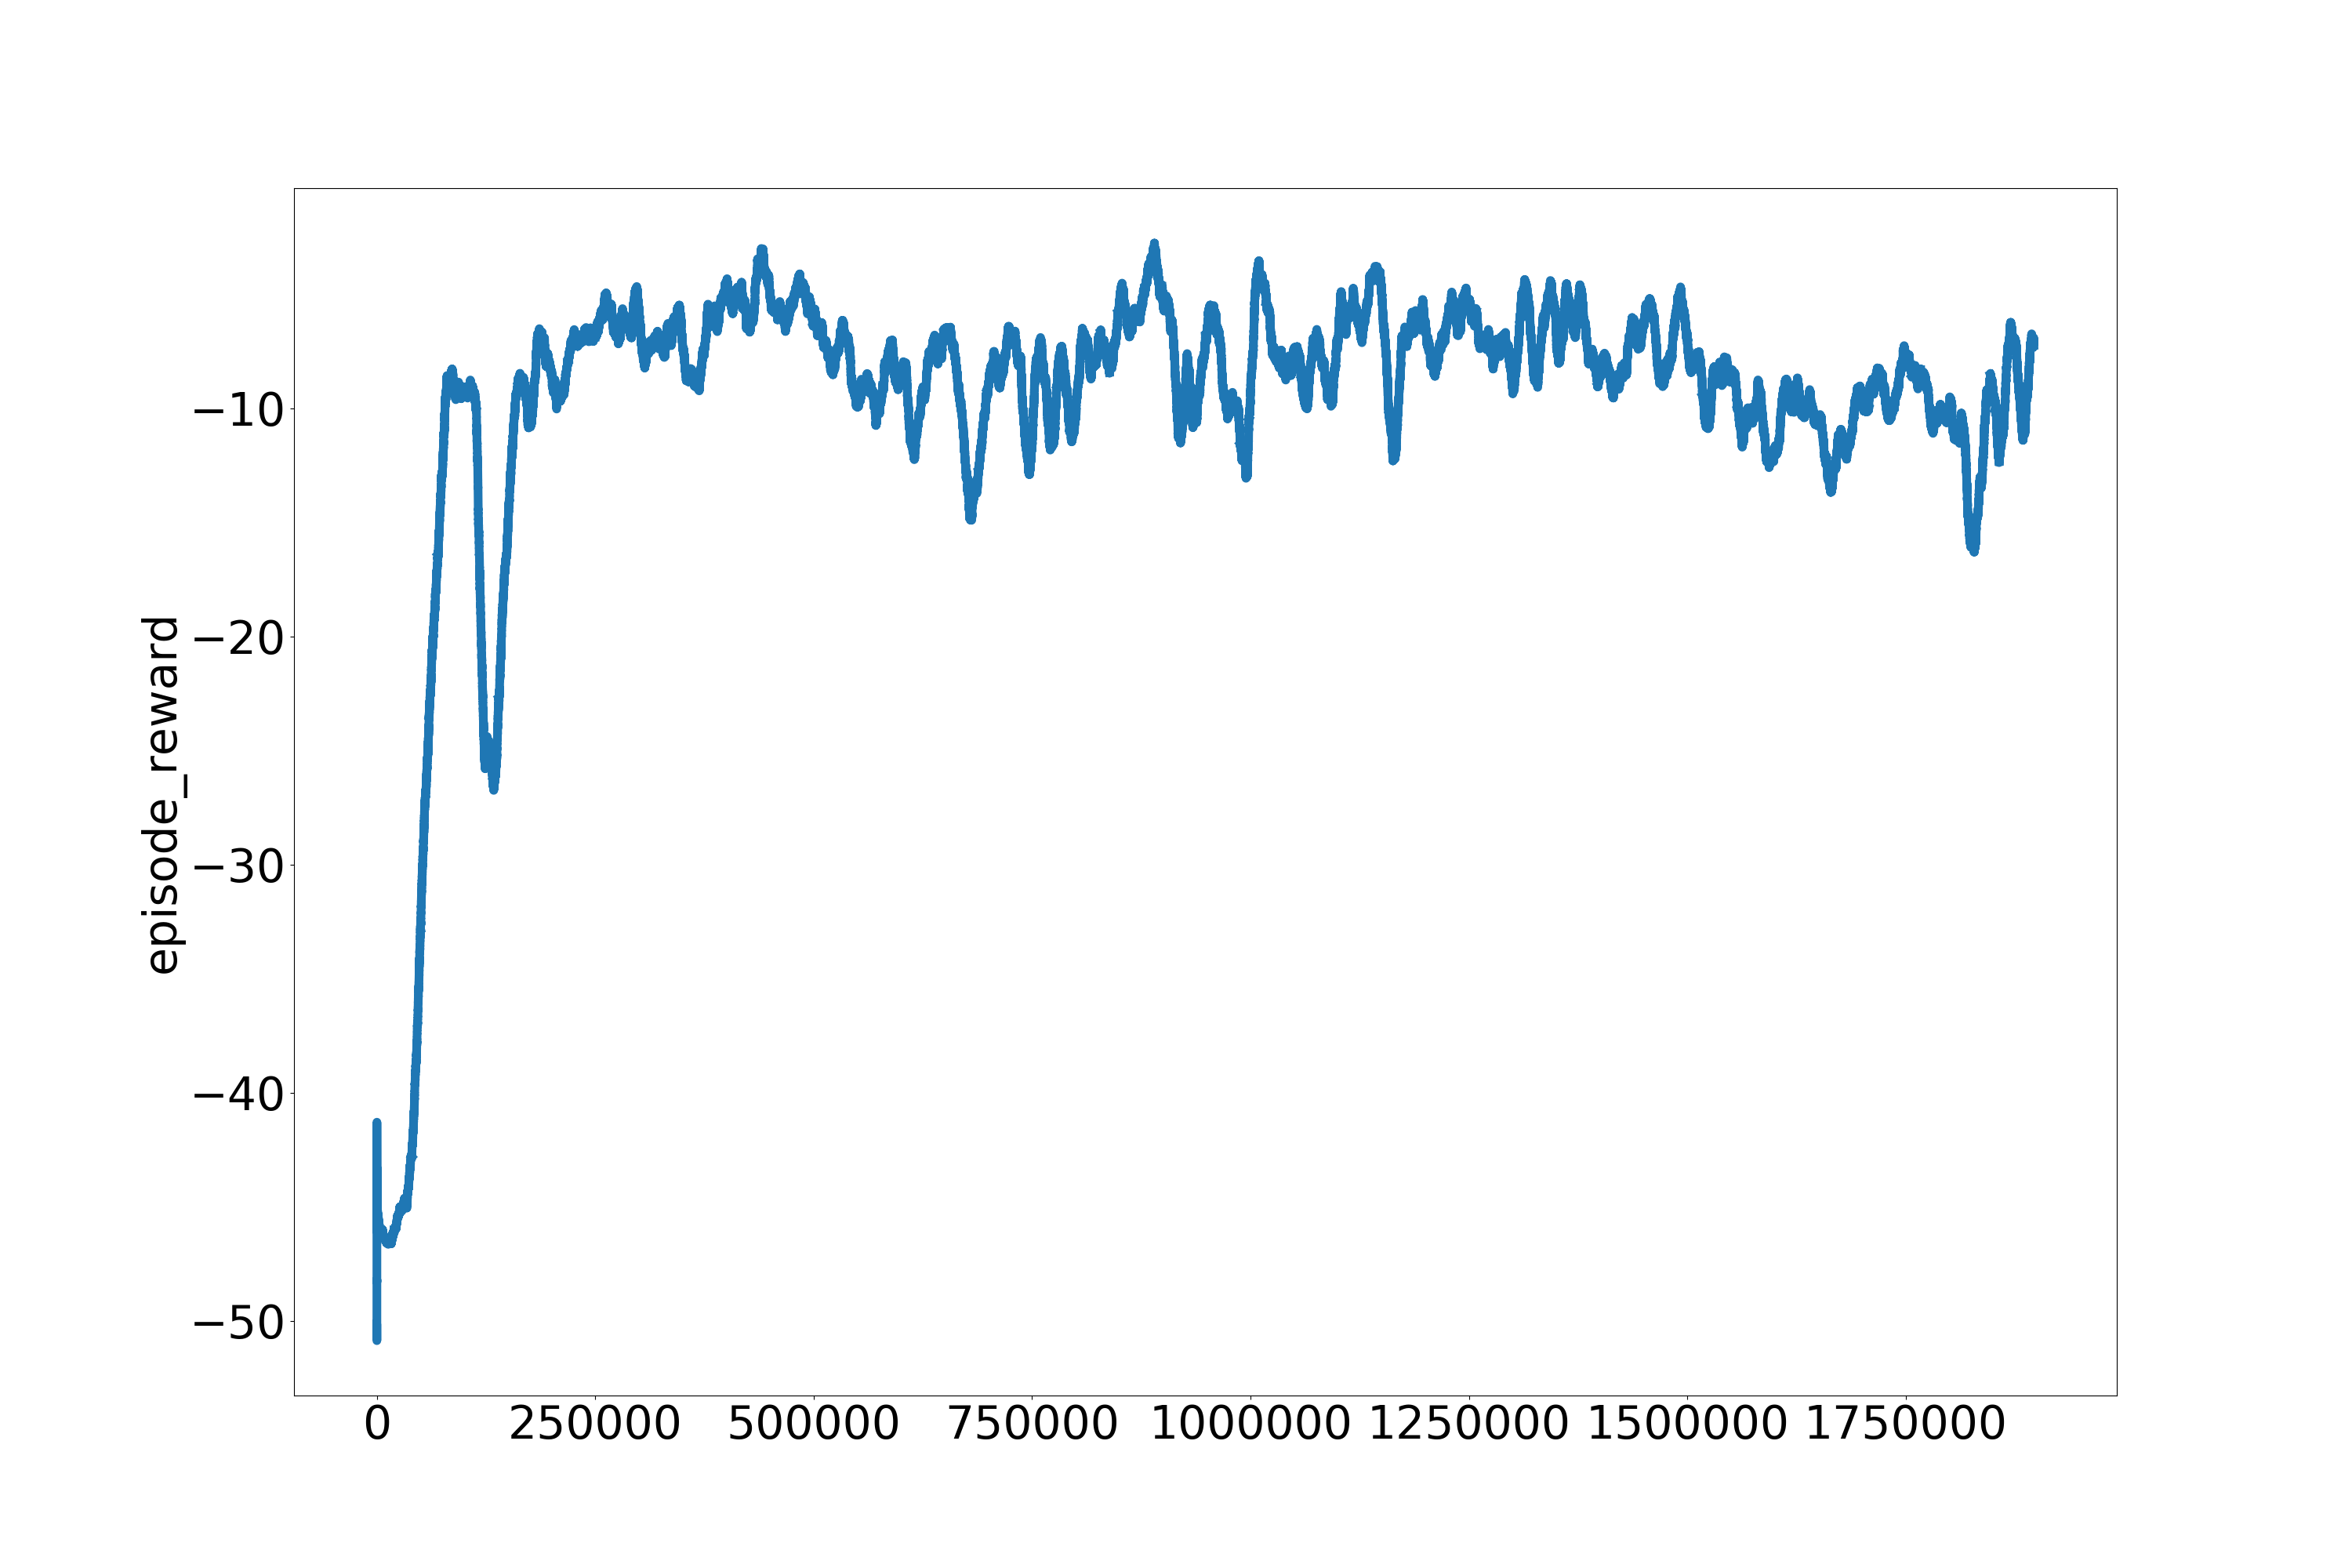
\includegraphics[width=1.1\textwidth]{Pic/First_model_50_reward/episode_reward.png}
      \caption{Trung bình tích lũy phần thưởng}
      \label{fig:first_model:try_2:avg}
    \end{subfigure}%
    \begin{subfigure}{.5\textwidth}
      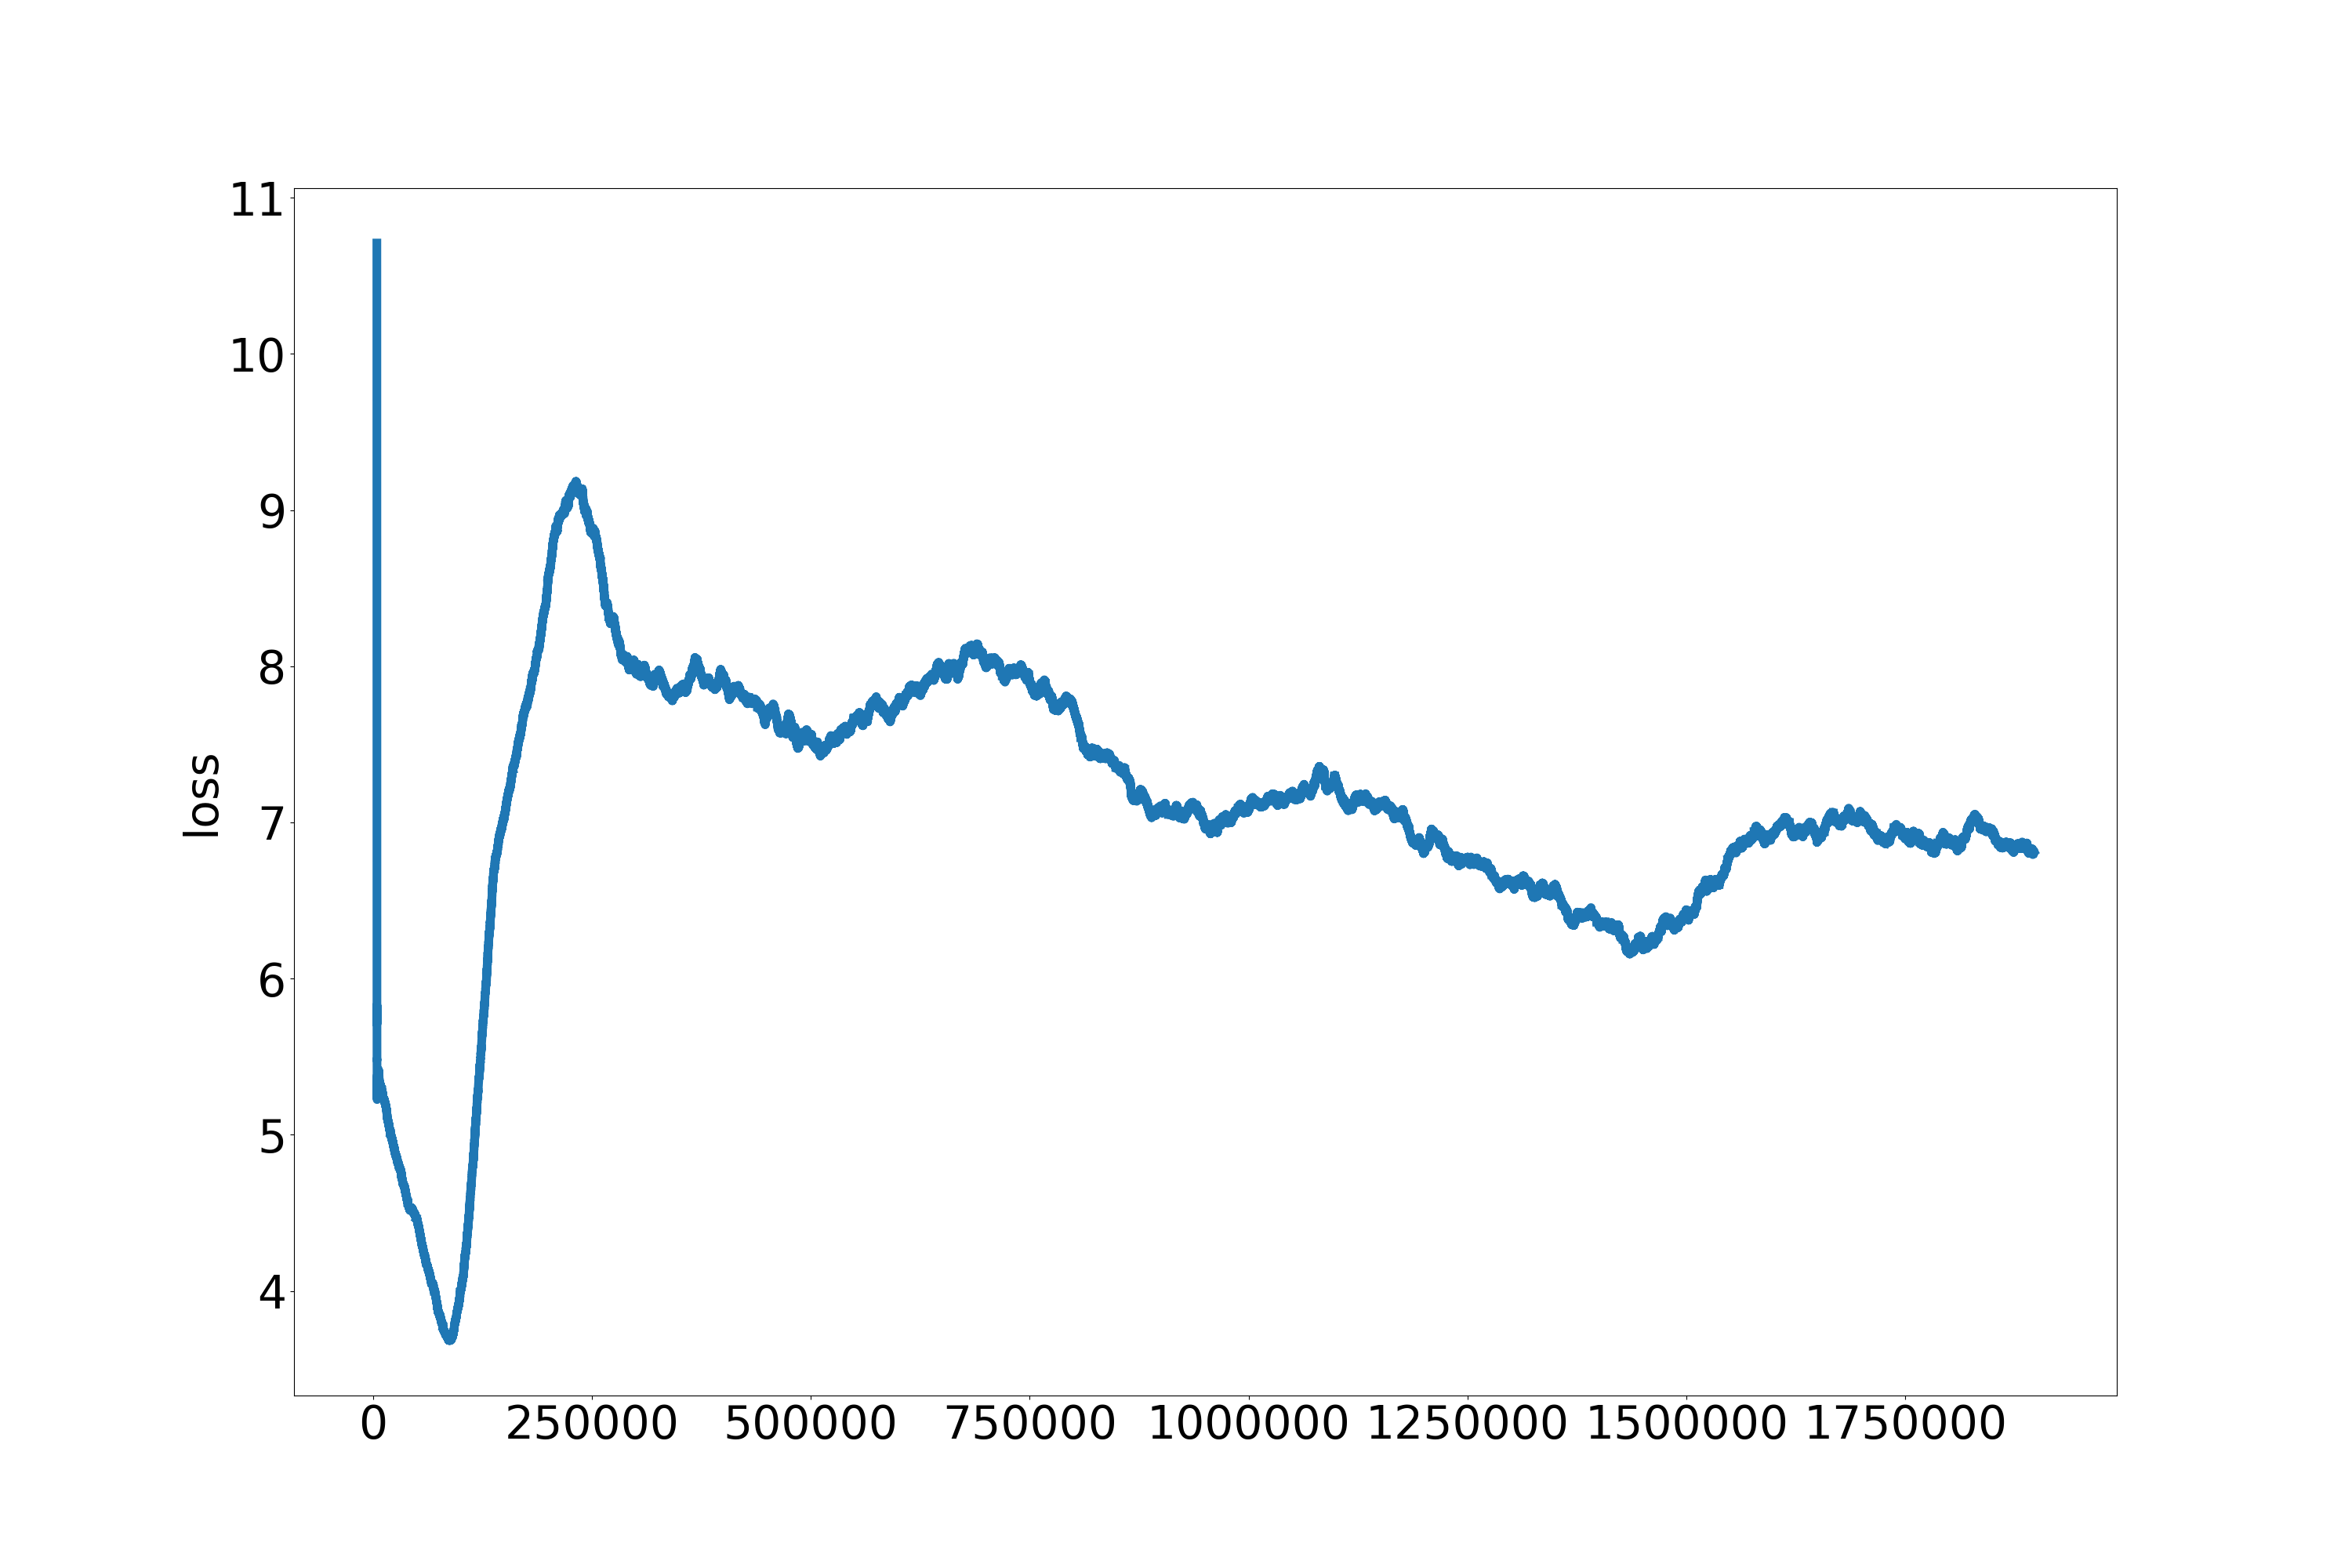
\includegraphics[width=1.1\textwidth]{Pic/First_model_50_reward/loss.png}
      \caption{Hàm mất mát}
      \label{fig:first_model:try_2:loss}
    \end{subfigure}
    \begin{subfigure}{.5\textwidth}
      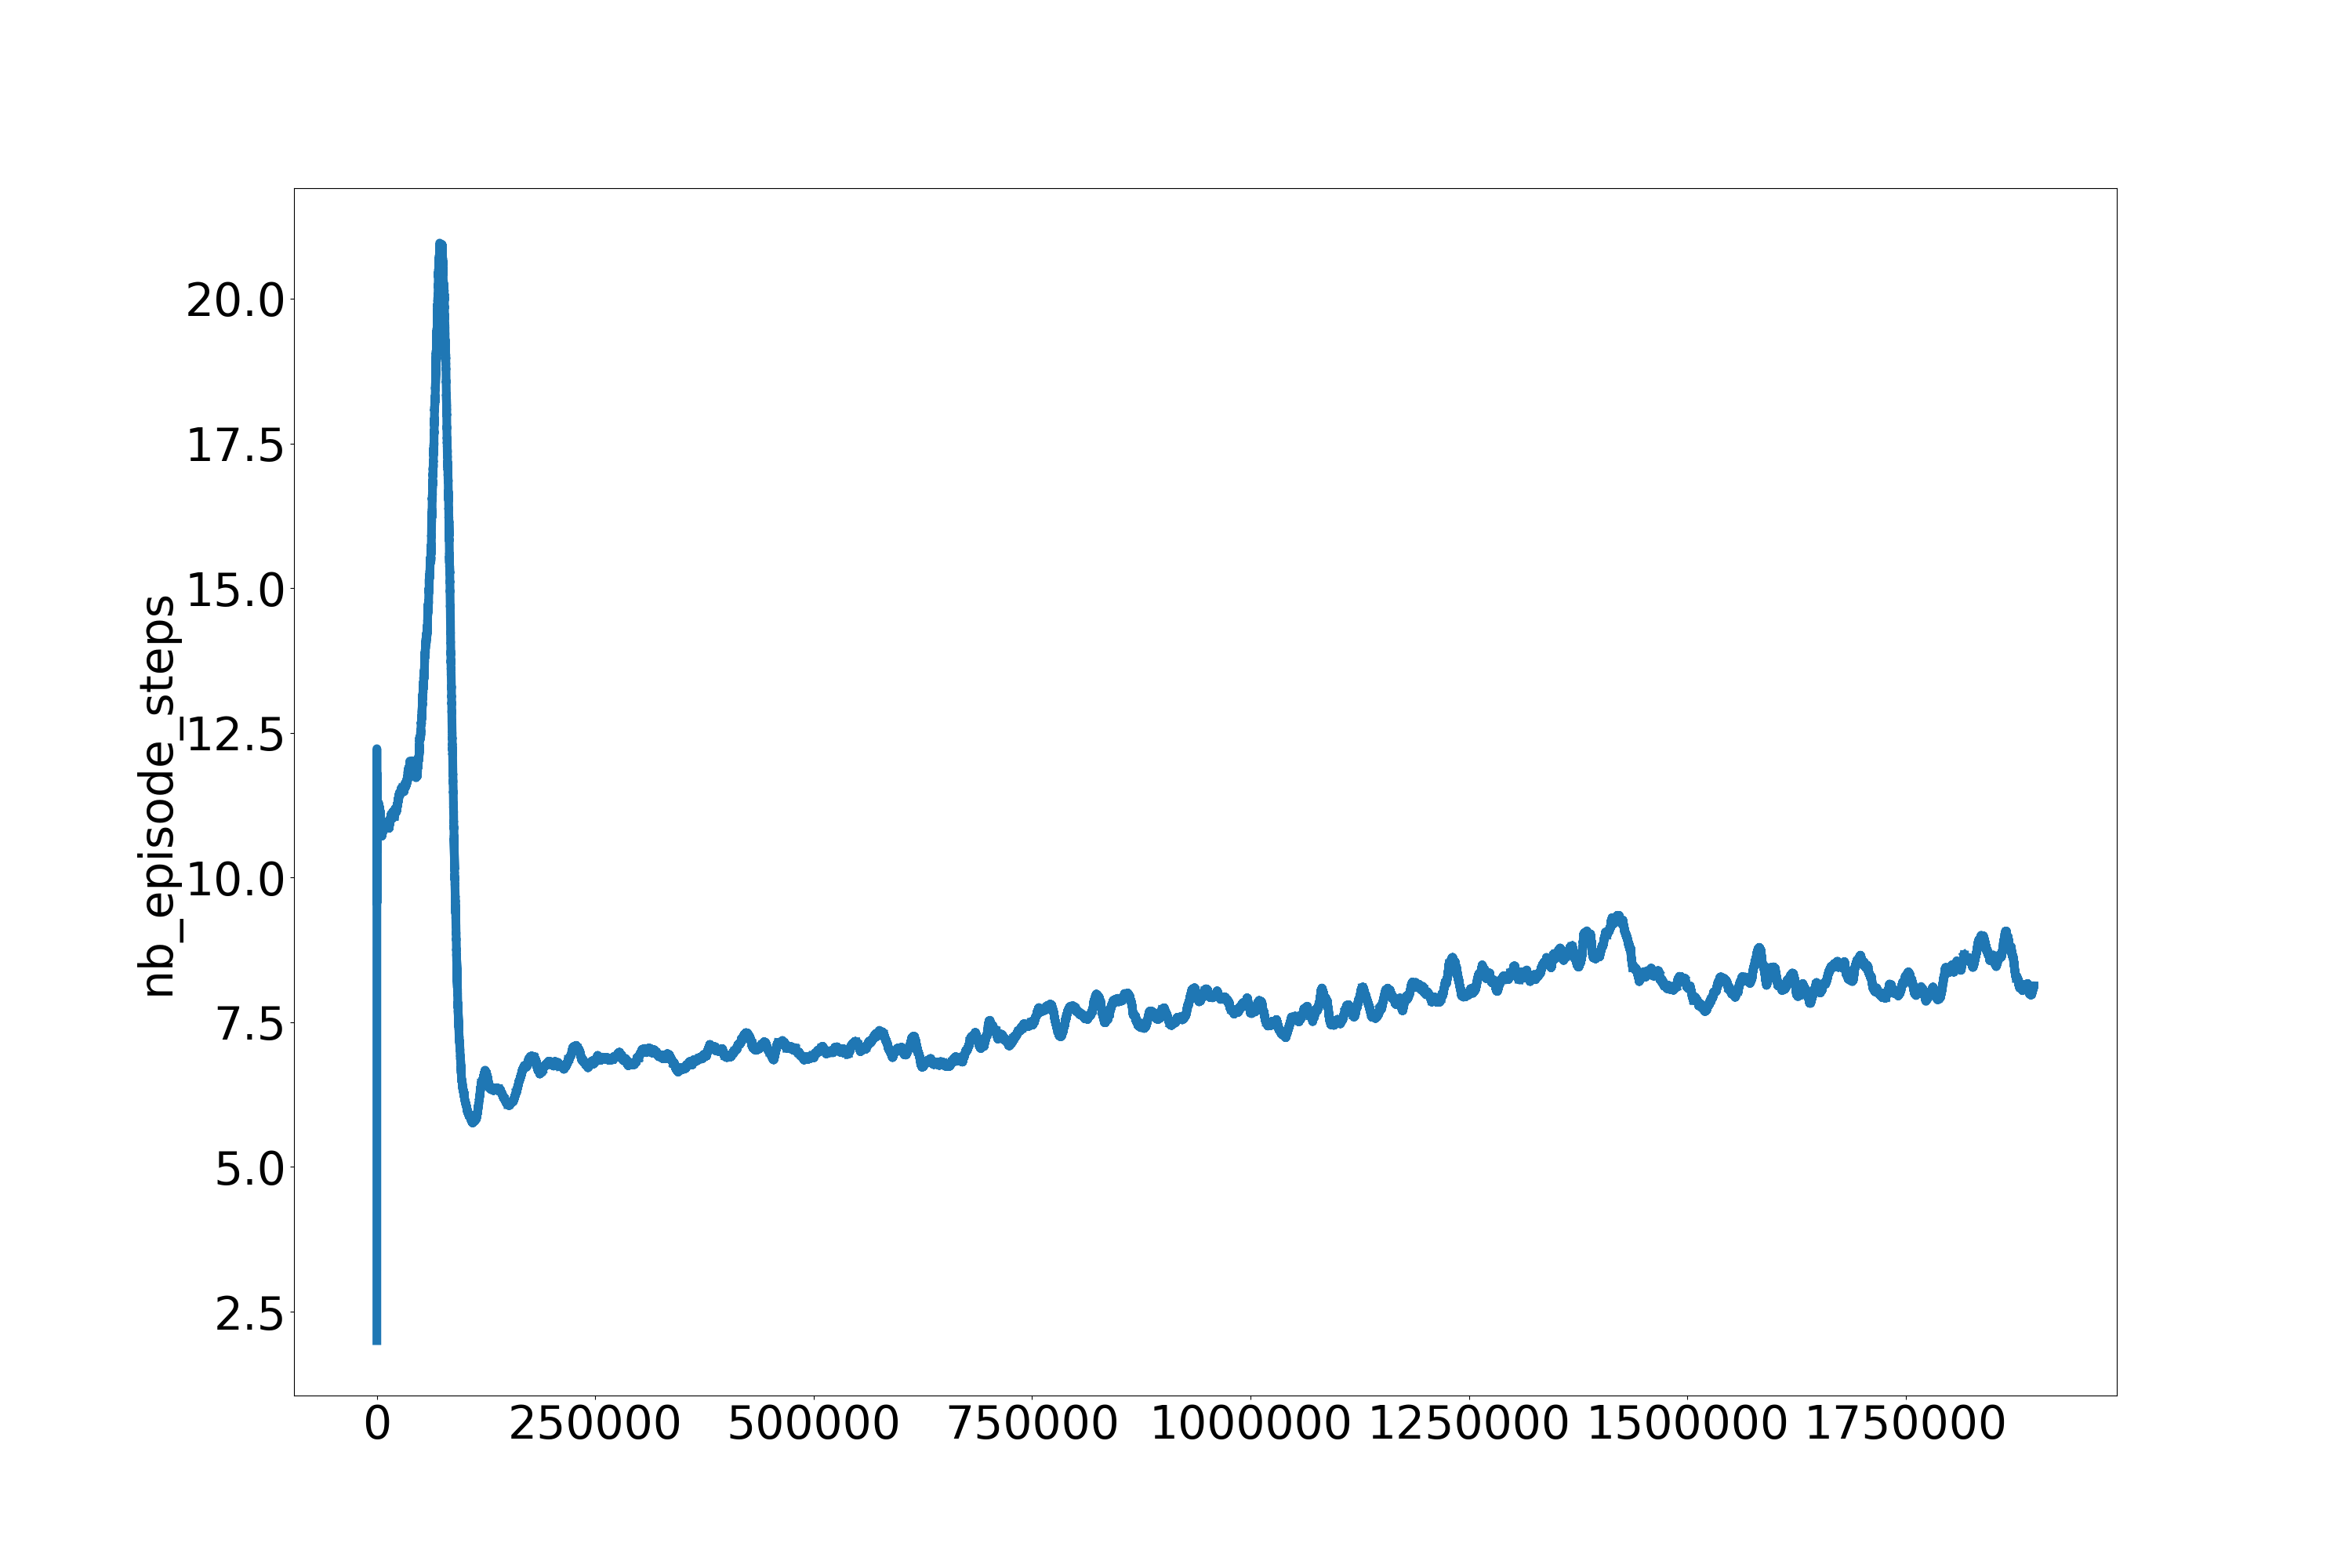
\includegraphics[width=1.1\textwidth]{Pic/First_model_50_reward/nb_episode_steps.png}
      \caption{Số bước thực hiện}
      \label{fig:first_model:try_2:step}
    \end{subfigure}%
    \begin{subfigure}{.5\textwidth}
      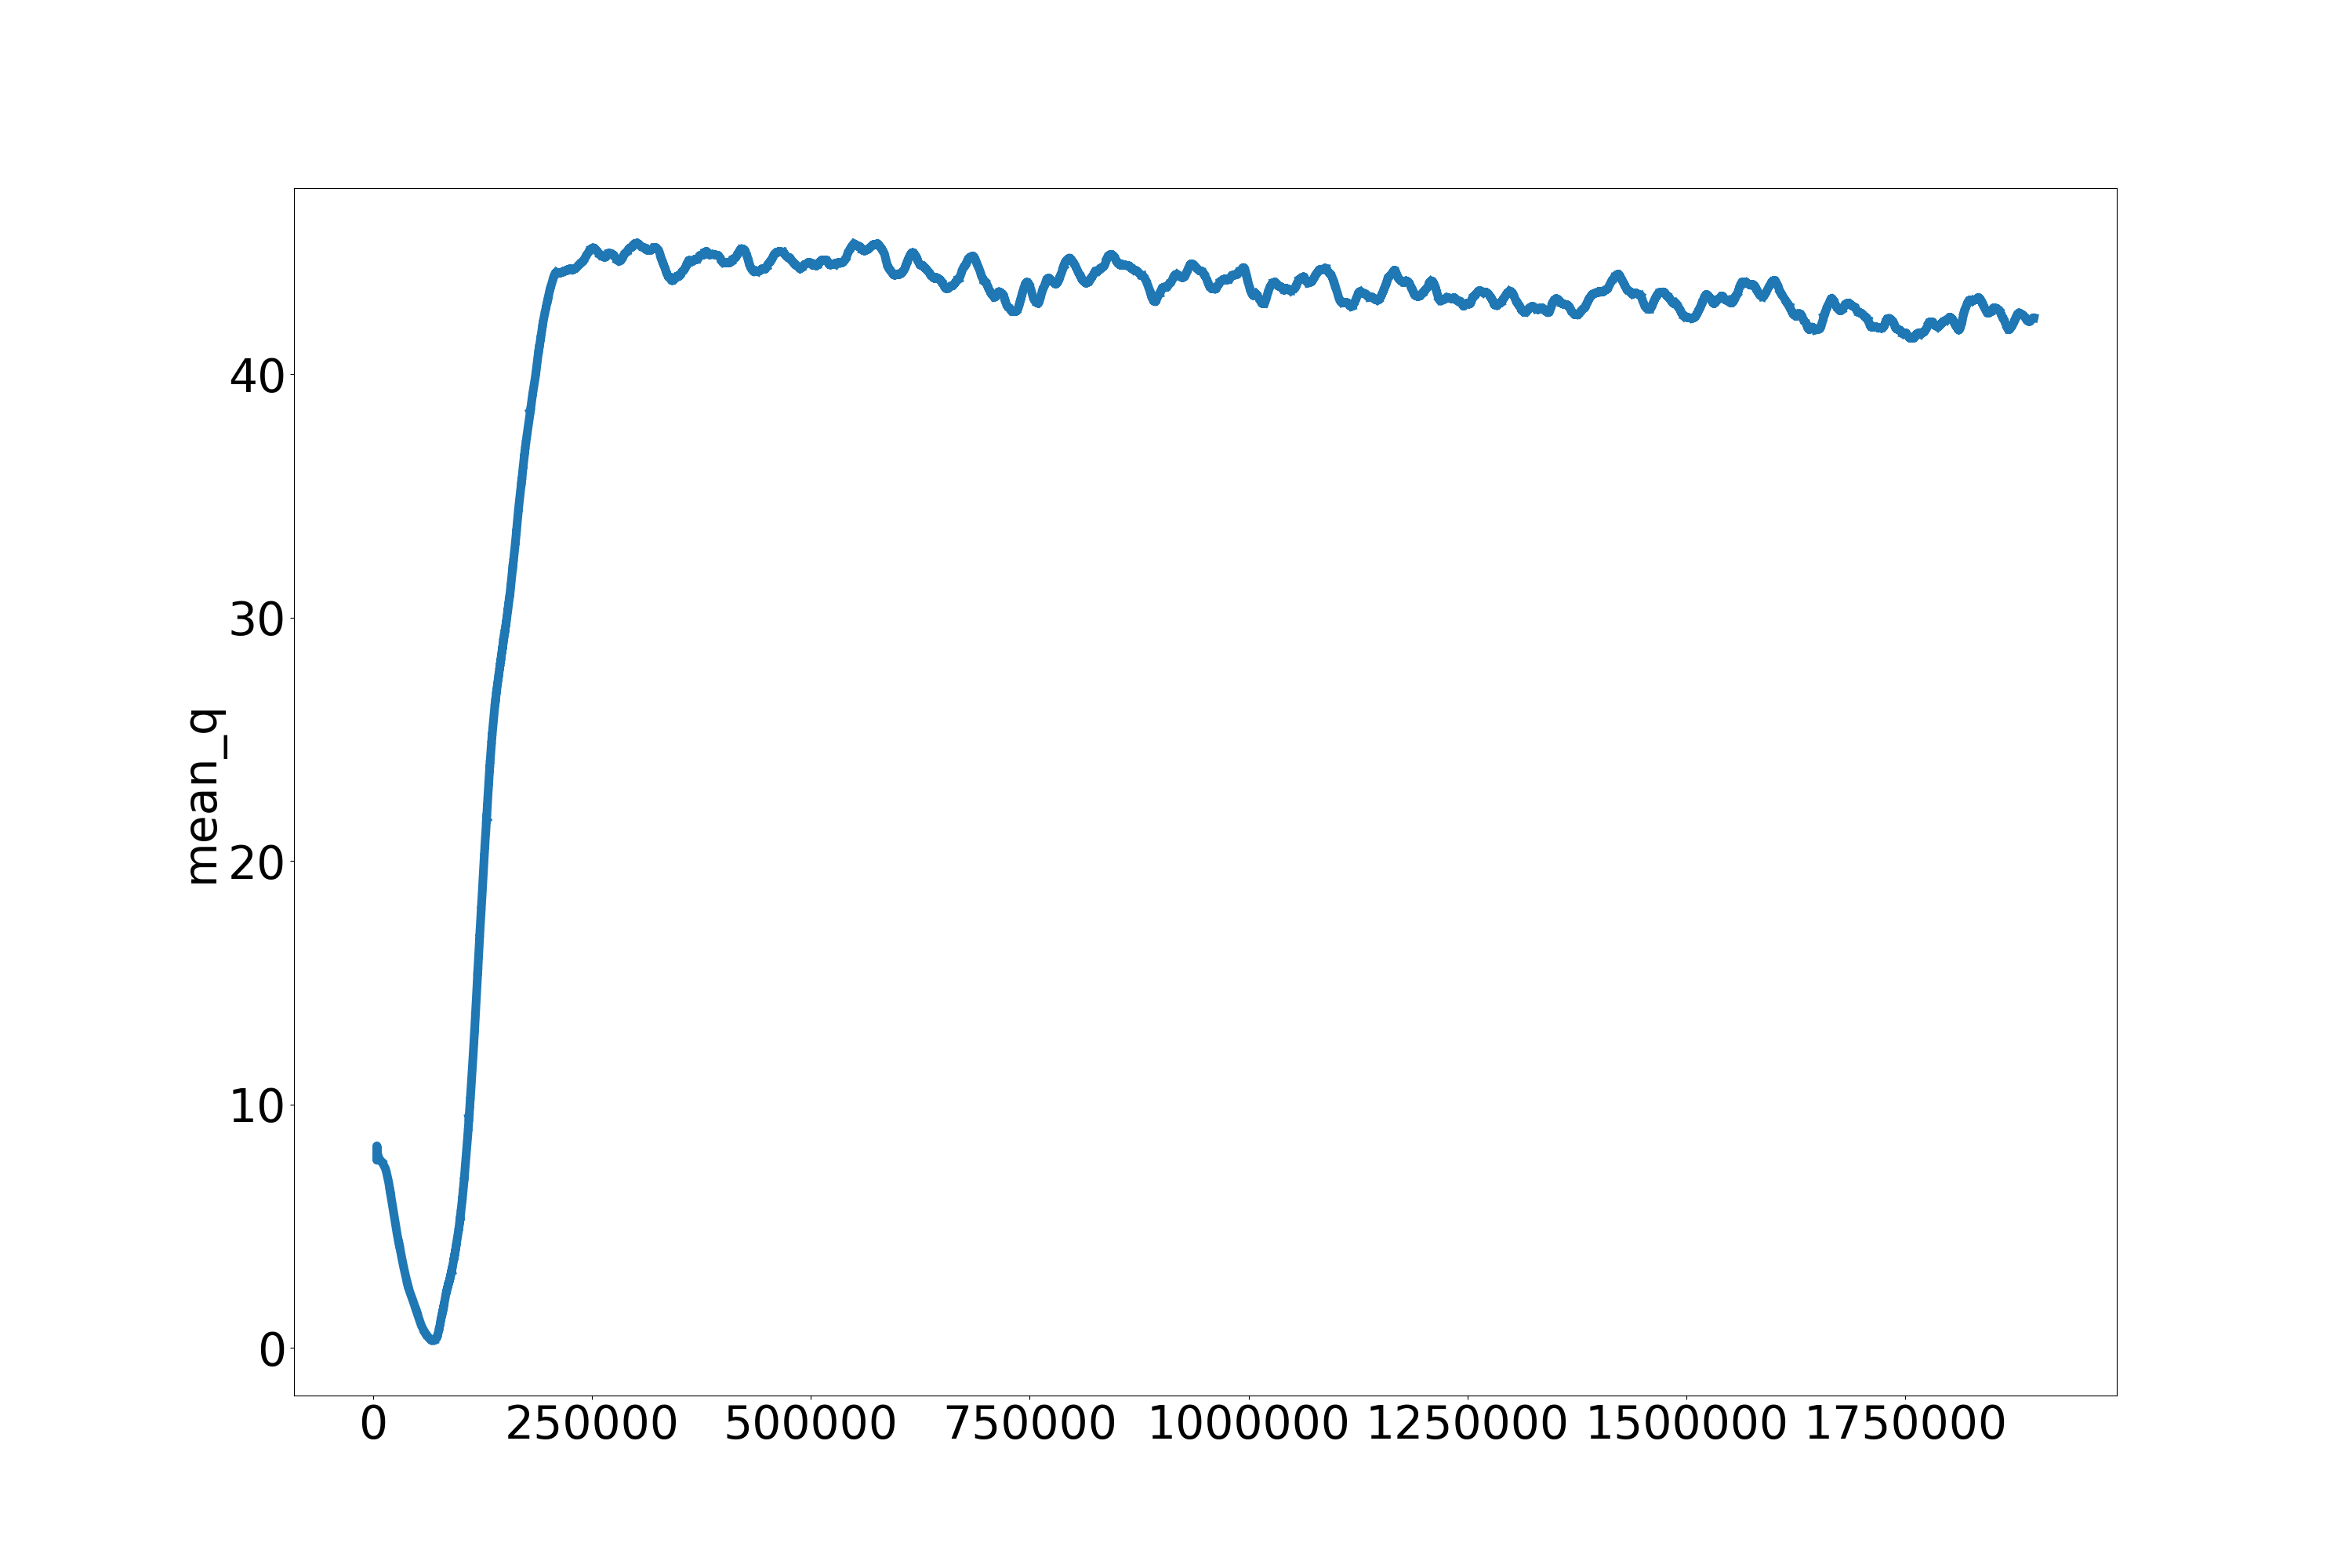
\includegraphics[width=1.1\textwidth]{Pic/First_model_50_reward/mean_q.png}
      \caption{Trung bình giá trị Q}
      \label{fig:first_model:try_2:mean_q}
    \end{subfigure}
\caption[Kết quả của mô hình thứ nhất lần hai]{\textit{Kết quả của mô hình thứ nhất lần hai}, thực nghiệm mô hình thứ hai chứng minh rằng khó có thể đạt được kết quả cao hơn được vì mô hình đã chạm mức "cực đại" của nó.}
\label{fig:result_first_model:try_2}
\end{figure}
\clearpage
\subsection{Mô hình thứ hai}
Dựa vào kết quả của mô hình thứ hai \ref{second_model}, sau hơn 6M bước được thực hiện, so sánh các với thực nghiệm [\ref{fig:result_first_model:try_1}, \ref{fig:result_first_model:try_2}] nhận xét đồ thị khá giống hình dáng nhau. Tuy nhiên khi xét đến trung bình giá trị Q của \ref{fig:result_first_model:try_1} và \ref{fig:resut_second_model}, có thể thấy đồ thị\ref{fig:resut_second_model:mean_q} đã đạt mốc cao hơn trên 7, điều này chứng tỏ mô hình thứ hai đã có cải tiến. Tỷ lệ thắng của mô hình đã chứng tỏ điều này khi đạt \textbf{55.8\%} (lưu ý rằng chỉ mới hơn 6M bước so với 14M bước). Đây là tín hiệu tích cực cho thấy mô hình thứ hai đã có những kết quả tốt hơn và vẫn còn có thể tiếp tục cải thiện khi thực hiện việc huấn luyện thêm nữa.
\begin{figure}[ht]
    \centering
    \begin{subfigure}{.5\textwidth}
      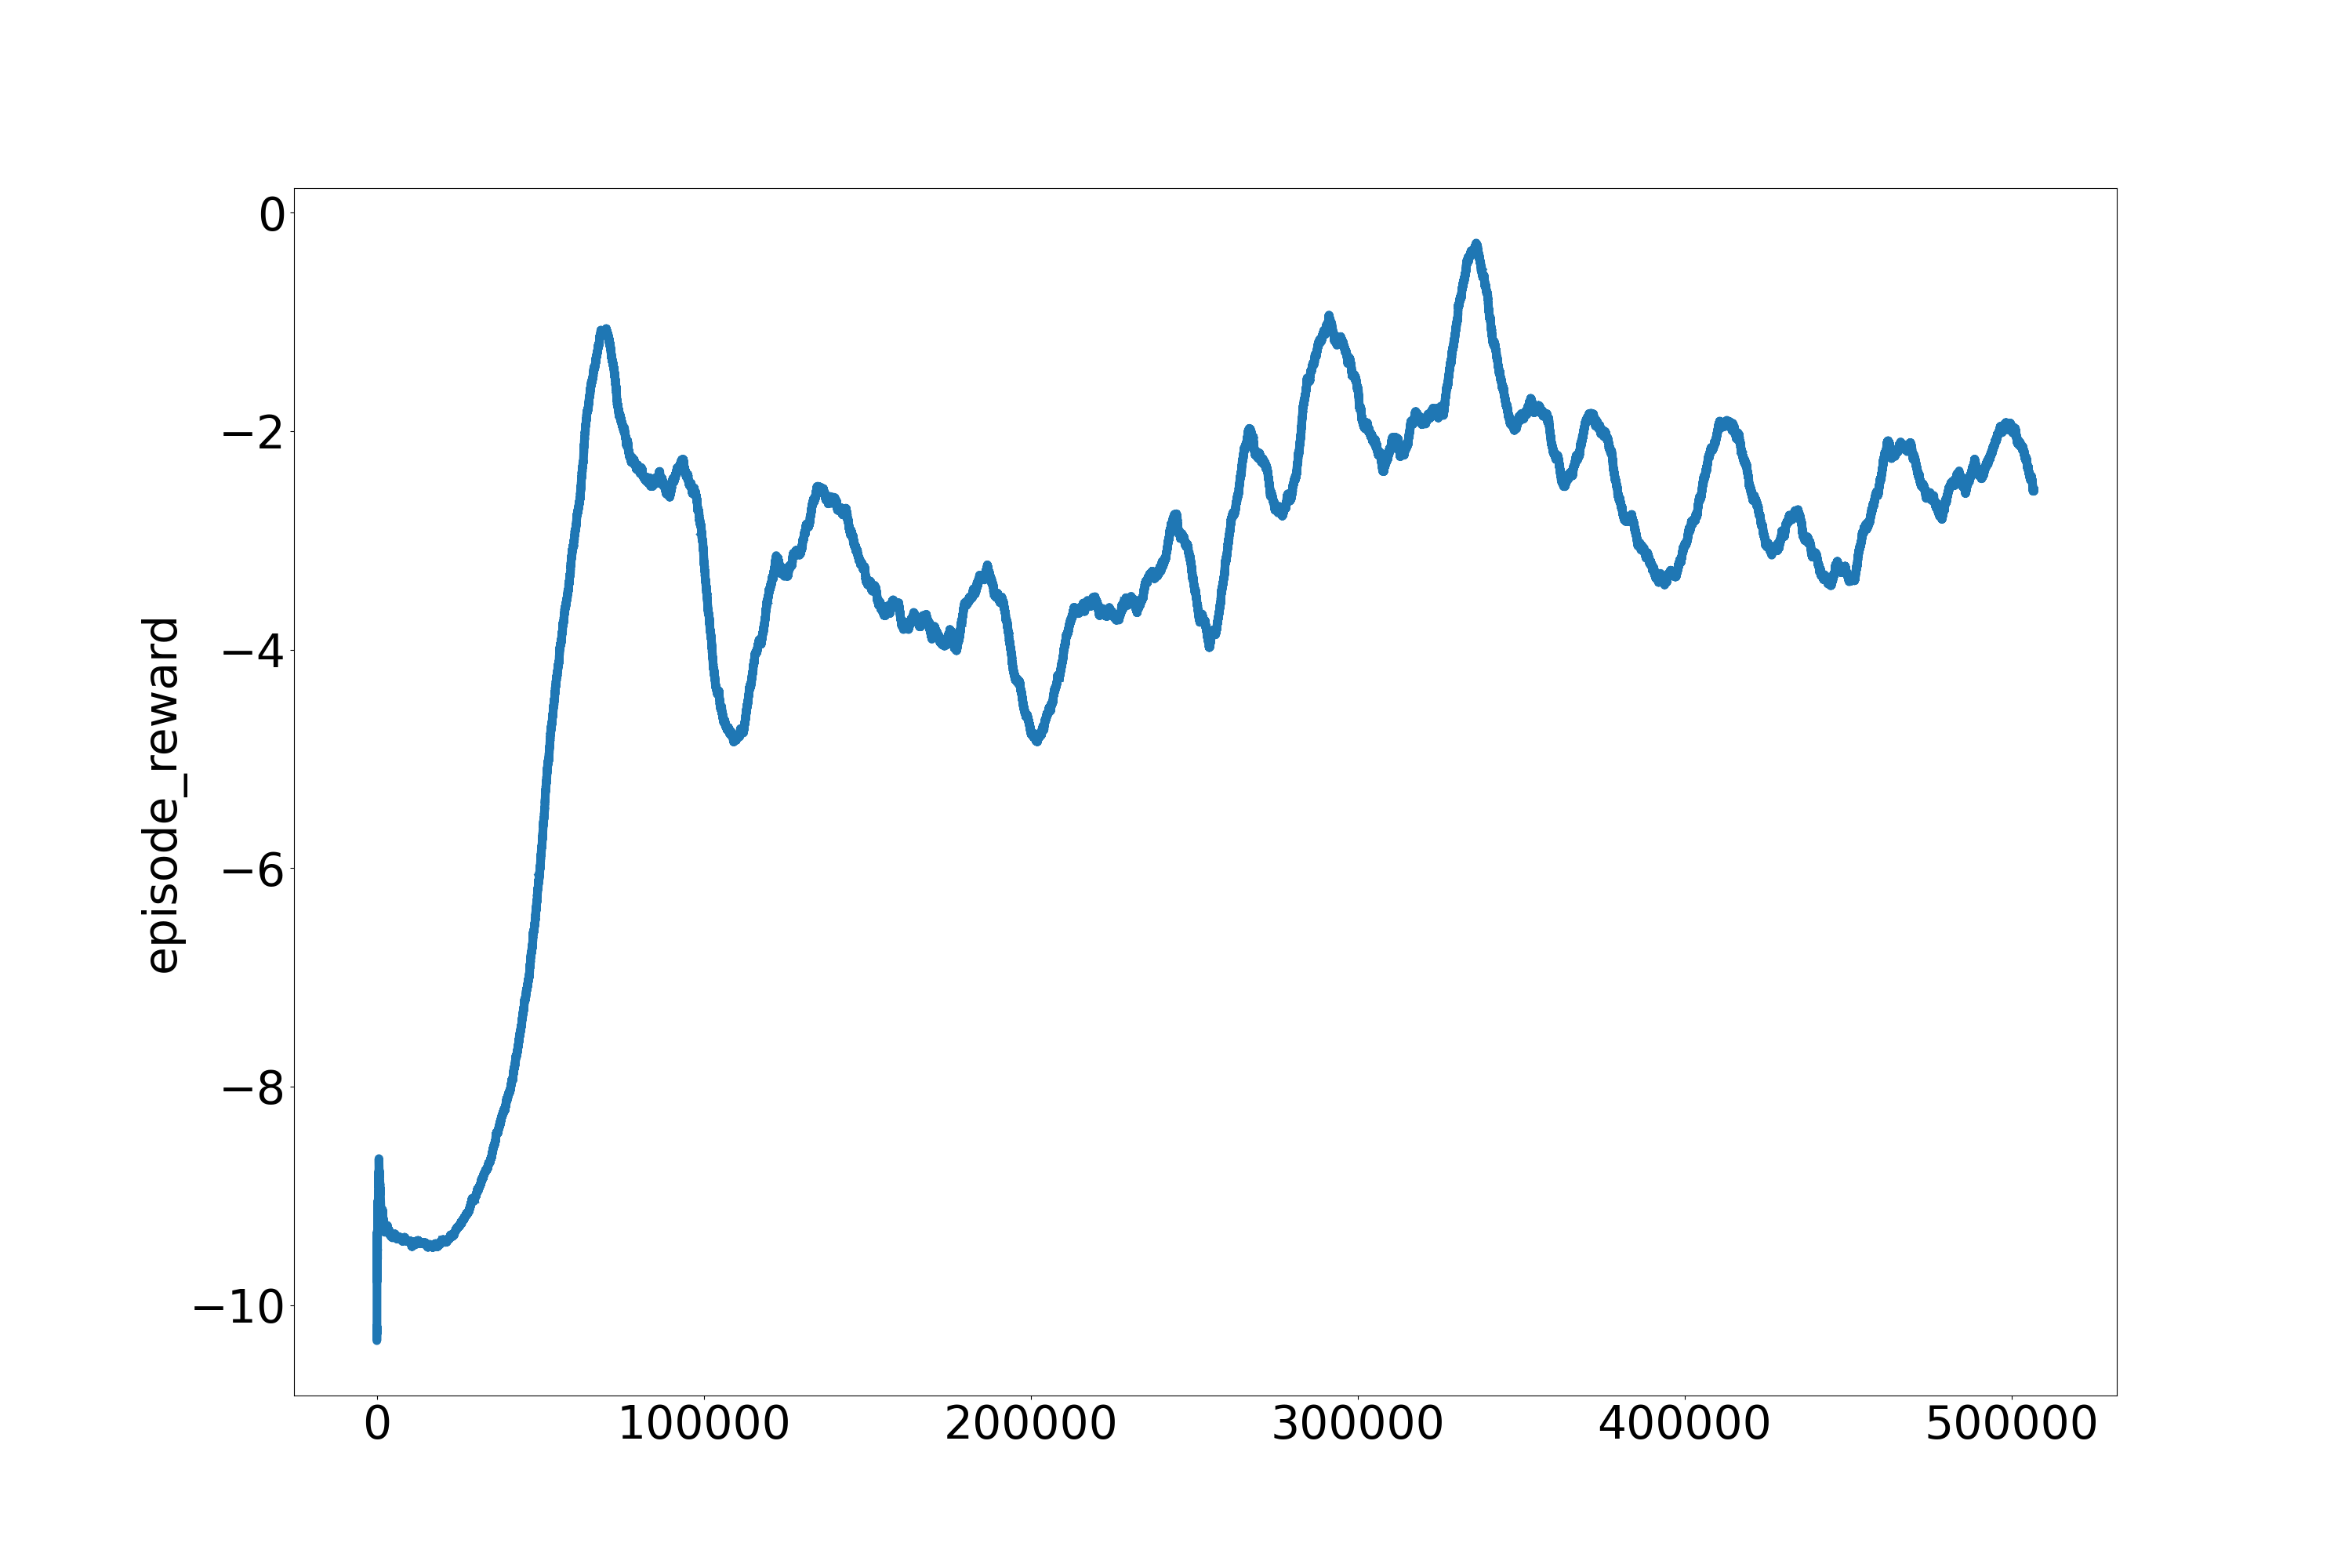
\includegraphics[width=1.1\textwidth]{Pic/Second_model/episode_reward.png}  
      \caption{Trung bình tích lũy phần thưởng}
      \label{fig:resut_second_model:avg}
    \end{subfigure}%
    \begin{subfigure}{.5\textwidth}
      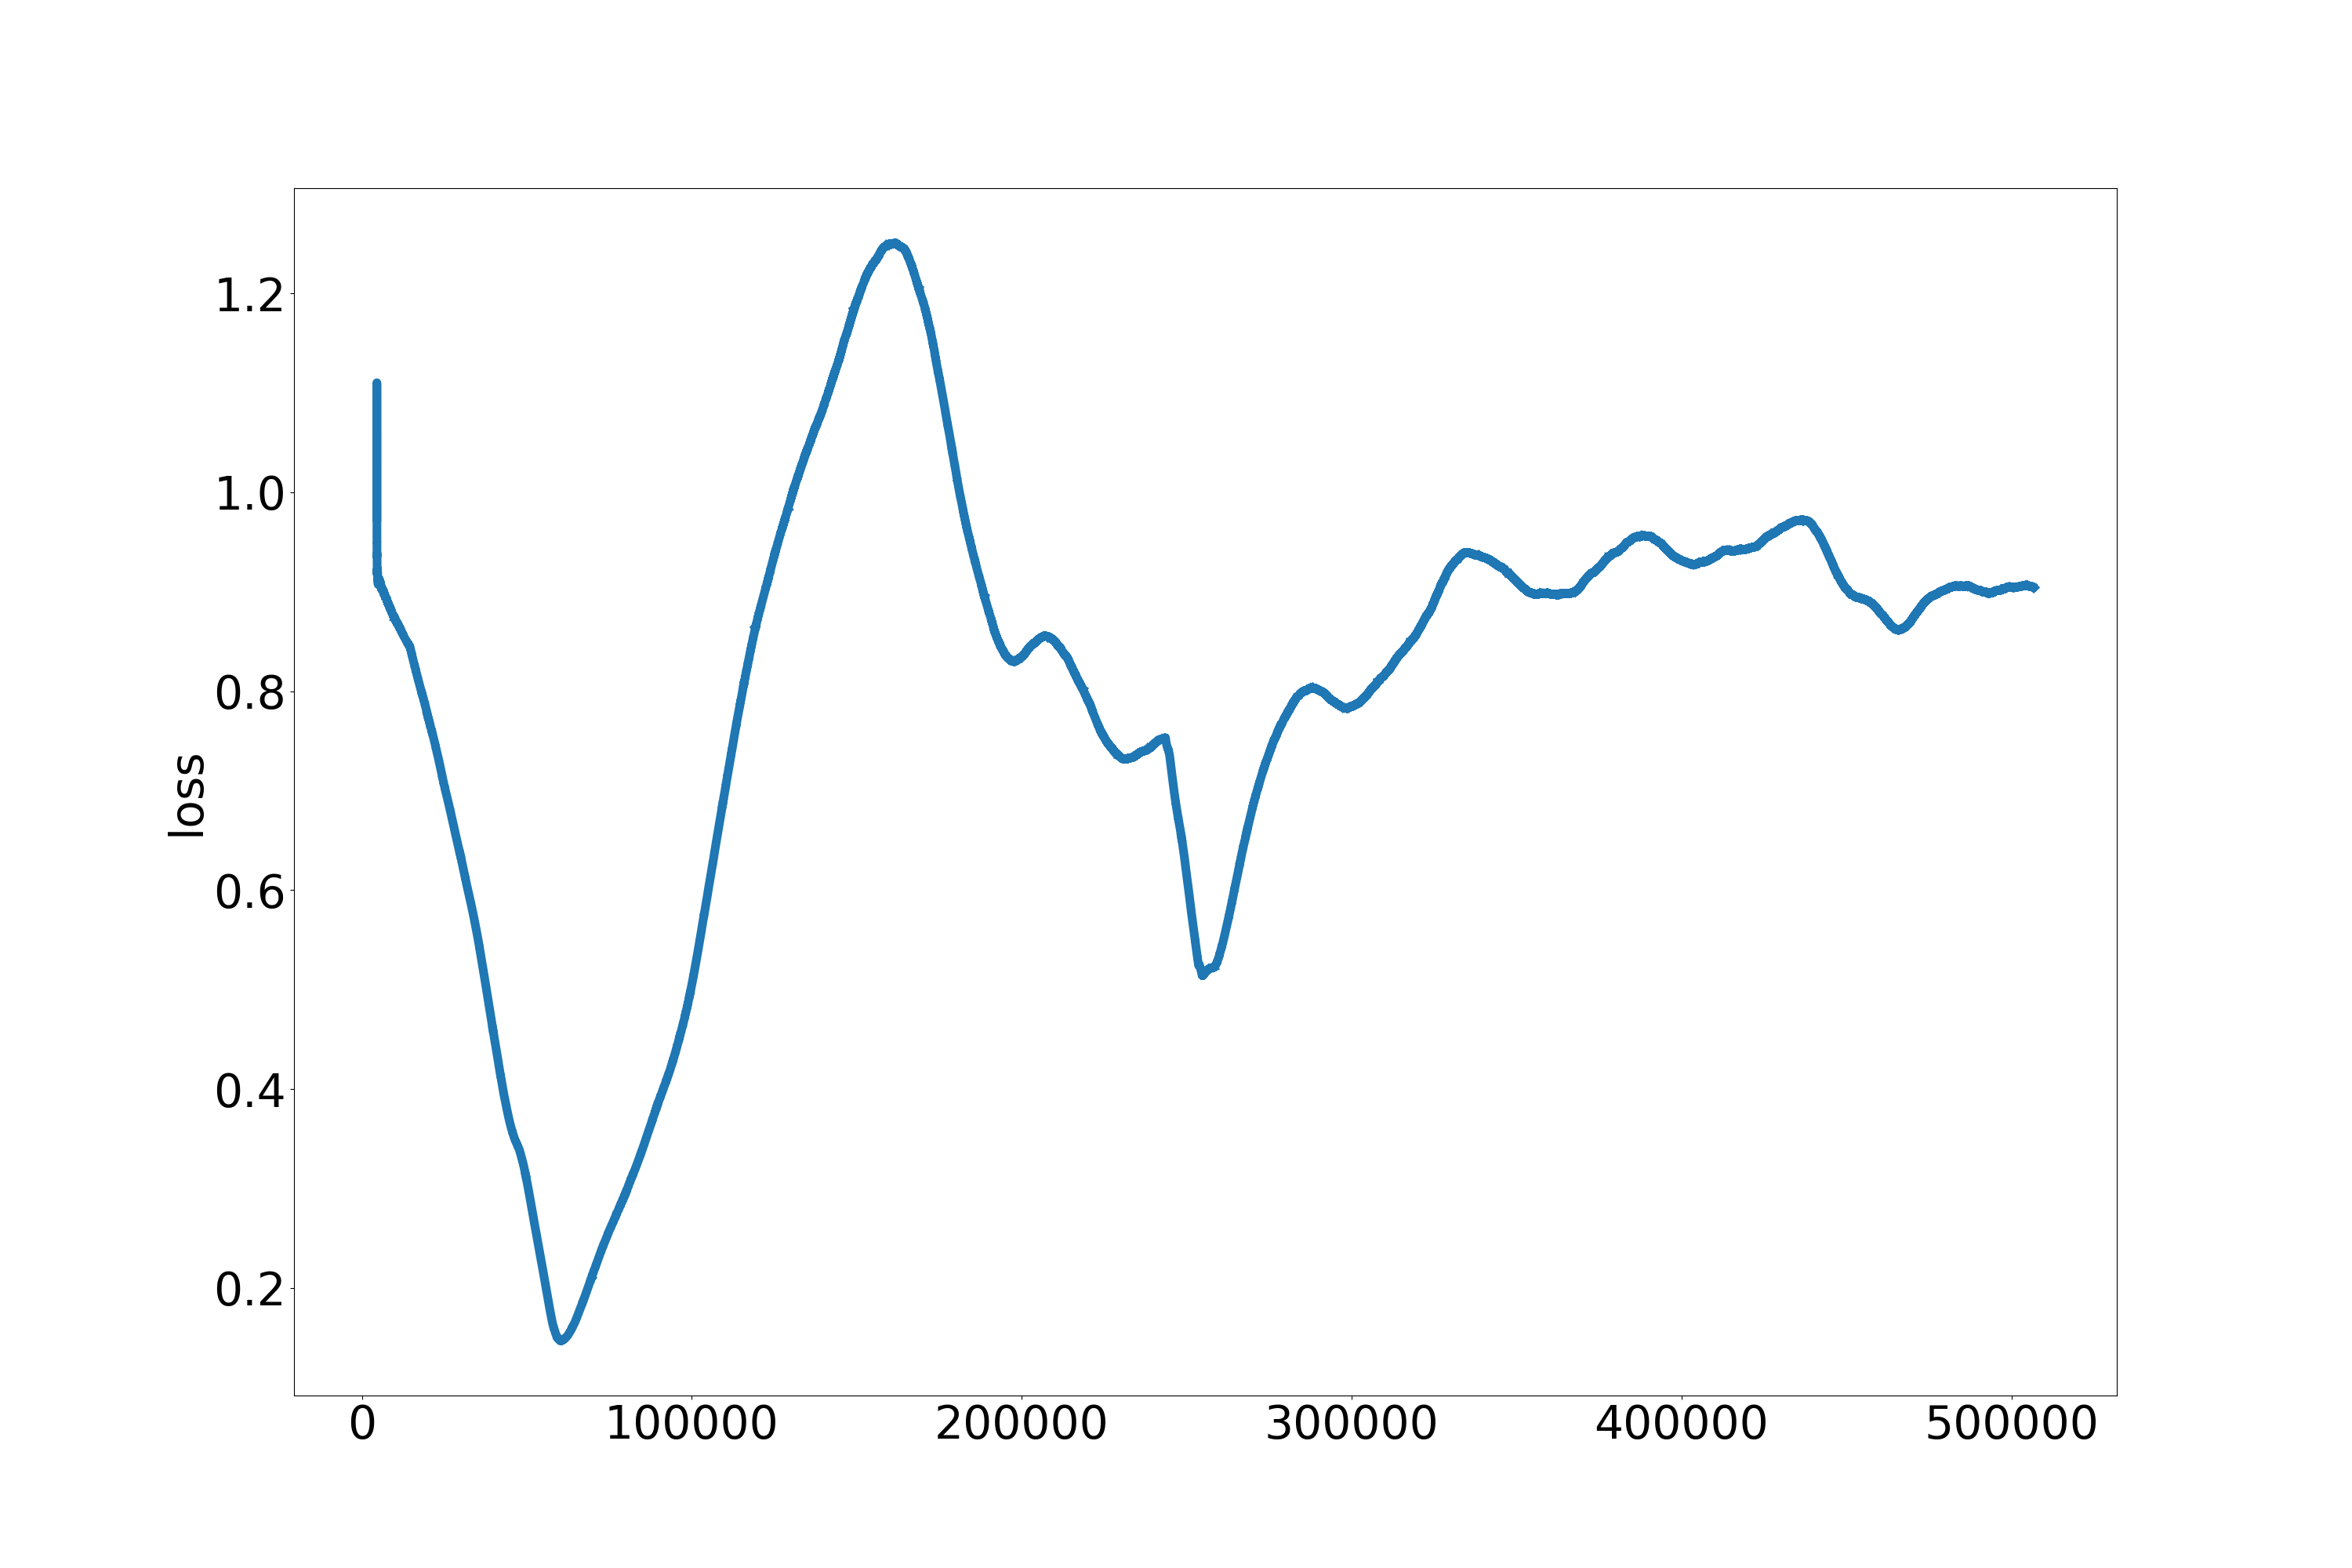
\includegraphics[width=1.1\textwidth]{Pic/Second_model/loss.png}  
      \caption{Hàm mất mát}
      \label{fig:resut_second_model:loss}
    \end{subfigure}\\
    \vspace{1cm}
    \begin{subfigure}{.5\textwidth}
      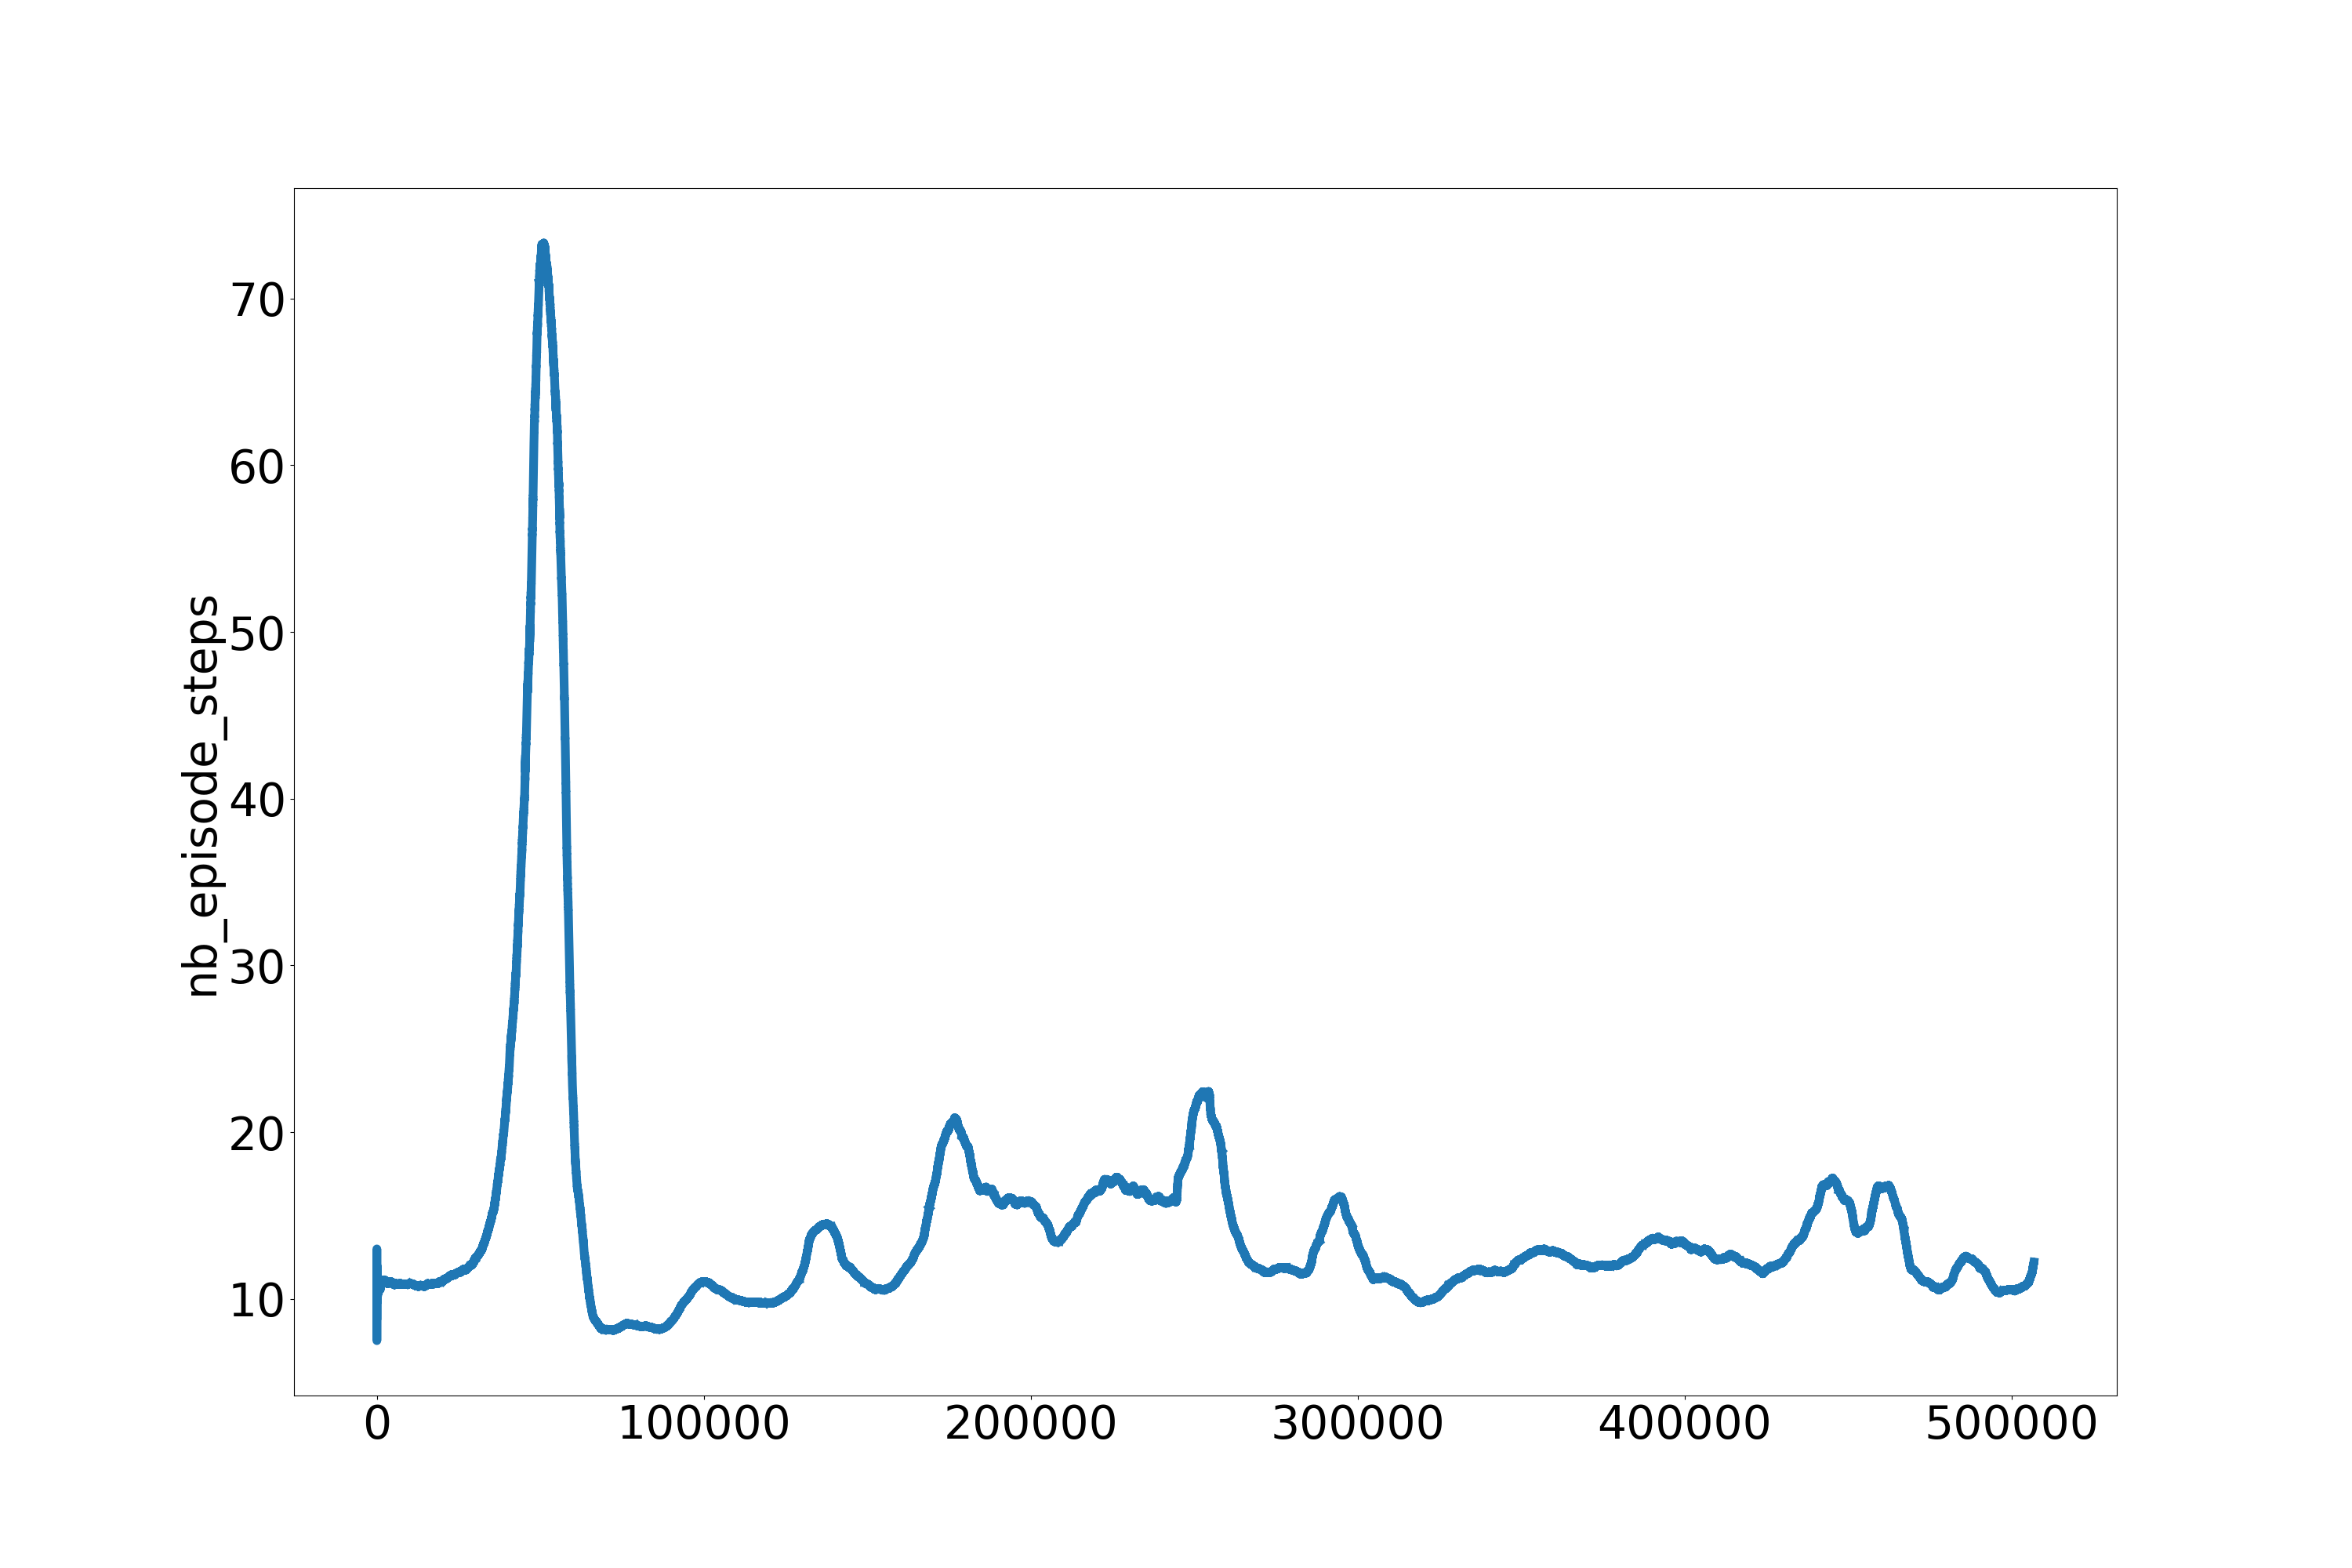
\includegraphics[width=1.1\textwidth]{Pic/Second_model/nb_episode_steps.png}
      \caption{Số bước thực hiện}
      \label{fig:resut_second_model:step}
    \end{subfigure}%
    \begin{subfigure}{.5\textwidth}
      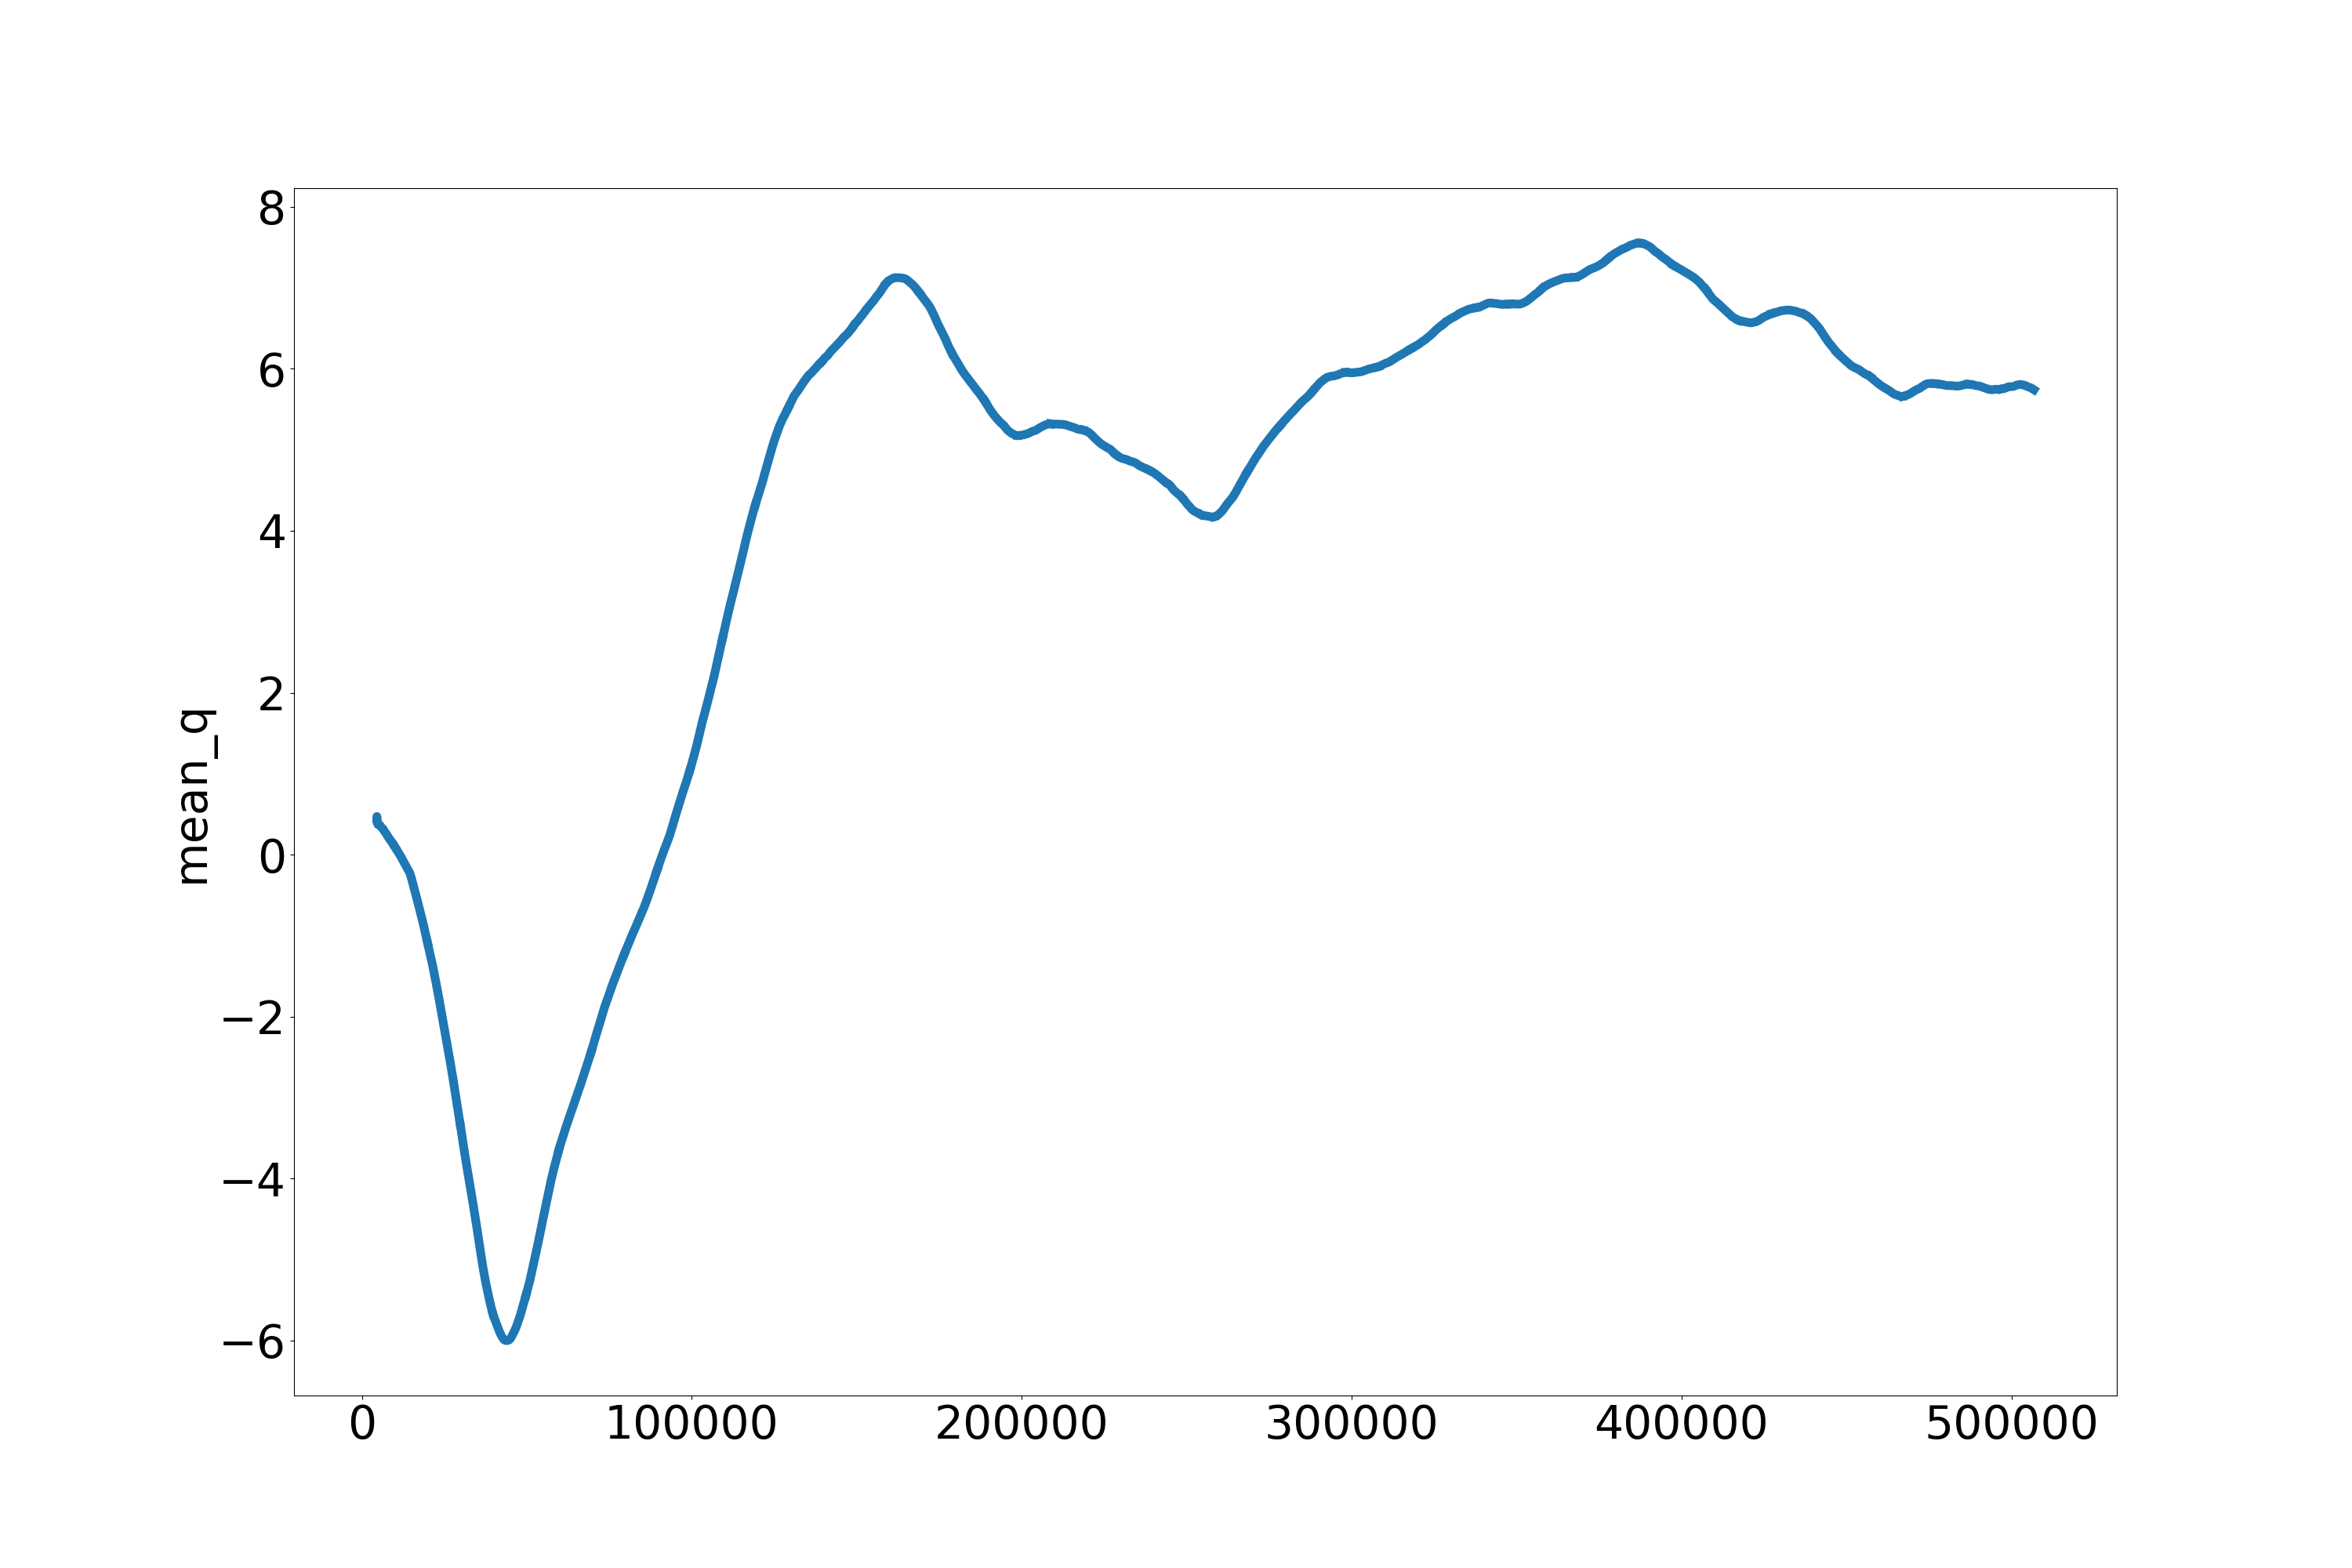
\includegraphics[width=1.1\textwidth]{Pic/Second_model/mean_q.png}  
      \caption{Trung bình giá trị Q}
      \label{fig:resut_second_model:mean_q}
    \end{subfigure}
\caption[Kết quả của mô hình thứ hai]{\textit{Kết quả của mô hình thứ hai}, có thể thấy rằng trung bình tích lũy phần thưởng chưa tăng lên vẫn còn dưới giá trị không tuy nhiên hàm mất mát chưa hội tụ và trung bình giá trị Q đạt được giá trị cao hơn so với \ref{fig:first_model:try1:mean_q}, điều này chứng tỏ mô hình vẫn có thể tốt hơn.}
\label{fig:resut_second_model}
\end{figure}
\newpage